
\documentclass{article} % For LaTeX2e
\usepackage{iclr2025_conference,times}

% Optional math commands from https://github.com/goodfeli/dlbook_notation.
%%%%% NEW MATH DEFINITIONS %%%%%

\usepackage{amsmath,amsfonts,bm}
\usepackage{derivative}
% Mark sections of captions for referring to divisions of figures
\newcommand{\figleft}{{\em (Left)}}
\newcommand{\figcenter}{{\em (Center)}}
\newcommand{\figright}{{\em (Right)}}
\newcommand{\figtop}{{\em (Top)}}
\newcommand{\figbottom}{{\em (Bottom)}}
\newcommand{\captiona}{{\em (a)}}
\newcommand{\captionb}{{\em (b)}}
\newcommand{\captionc}{{\em (c)}}
\newcommand{\captiond}{{\em (d)}}

% Highlight a newly defined term
\newcommand{\newterm}[1]{{\bf #1}}

% Derivative d 
\newcommand{\deriv}{{\mathrm{d}}}

% Figure reference, lower-case.
\def\figref#1{figure~\ref{#1}}
% Figure reference, capital. For start of sentence
\def\Figref#1{Figure~\ref{#1}}
\def\twofigref#1#2{figures \ref{#1} and \ref{#2}}
\def\quadfigref#1#2#3#4{figures \ref{#1}, \ref{#2}, \ref{#3} and \ref{#4}}
% Section reference, lower-case.
\def\secref#1{section~\ref{#1}}
% Section reference, capital.
\def\Secref#1{Section~\ref{#1}}
% Reference to two sections.
\def\twosecrefs#1#2{sections \ref{#1} and \ref{#2}}
% Reference to three sections.
\def\secrefs#1#2#3{sections \ref{#1}, \ref{#2} and \ref{#3}}
% Reference to an equation, lower-case.
\def\eqref#1{equation~\ref{#1}}
% Reference to an equation, upper case
\def\Eqref#1{Equation~\ref{#1}}
% A raw reference to an equation---avoid using if possible
\def\plaineqref#1{\ref{#1}}
% Reference to a chapter, lower-case.
\def\chapref#1{chapter~\ref{#1}}
% Reference to an equation, upper case.
\def\Chapref#1{Chapter~\ref{#1}}
% Reference to a range of chapters
\def\rangechapref#1#2{chapters\ref{#1}--\ref{#2}}
% Reference to an algorithm, lower-case.
\def\algref#1{algorithm~\ref{#1}}
% Reference to an algorithm, upper case.
\def\Algref#1{Algorithm~\ref{#1}}
\def\twoalgref#1#2{algorithms \ref{#1} and \ref{#2}}
\def\Twoalgref#1#2{Algorithms \ref{#1} and \ref{#2}}
% Reference to a part, lower case
\def\partref#1{part~\ref{#1}}
% Reference to a part, upper case
\def\Partref#1{Part~\ref{#1}}
\def\twopartref#1#2{parts \ref{#1} and \ref{#2}}

\def\ceil#1{\lceil #1 \rceil}
\def\floor#1{\lfloor #1 \rfloor}
\def\1{\bm{1}}
\newcommand{\train}{\mathcal{D}}
\newcommand{\valid}{\mathcal{D_{\mathrm{valid}}}}
\newcommand{\test}{\mathcal{D_{\mathrm{test}}}}

\def\eps{{\epsilon}}


% Random variables
\def\reta{{\textnormal{$\eta$}}}
\def\ra{{\textnormal{a}}}
\def\rb{{\textnormal{b}}}
\def\rc{{\textnormal{c}}}
\def\rd{{\textnormal{d}}}
\def\re{{\textnormal{e}}}
\def\rf{{\textnormal{f}}}
\def\rg{{\textnormal{g}}}
\def\rh{{\textnormal{h}}}
\def\ri{{\textnormal{i}}}
\def\rj{{\textnormal{j}}}
\def\rk{{\textnormal{k}}}
\def\rl{{\textnormal{l}}}
% rm is already a command, just don't name any random variables m
\def\rn{{\textnormal{n}}}
\def\ro{{\textnormal{o}}}
\def\rp{{\textnormal{p}}}
\def\rq{{\textnormal{q}}}
\def\rr{{\textnormal{r}}}
\def\rs{{\textnormal{s}}}
\def\rt{{\textnormal{t}}}
\def\ru{{\textnormal{u}}}
\def\rv{{\textnormal{v}}}
\def\rw{{\textnormal{w}}}
\def\rx{{\textnormal{x}}}
\def\ry{{\textnormal{y}}}
\def\rz{{\textnormal{z}}}

% Random vectors
\def\rvepsilon{{\mathbf{\epsilon}}}
\def\rvphi{{\mathbf{\phi}}}
\def\rvtheta{{\mathbf{\theta}}}
\def\rva{{\mathbf{a}}}
\def\rvb{{\mathbf{b}}}
\def\rvc{{\mathbf{c}}}
\def\rvd{{\mathbf{d}}}
\def\rve{{\mathbf{e}}}
\def\rvf{{\mathbf{f}}}
\def\rvg{{\mathbf{g}}}
\def\rvh{{\mathbf{h}}}
\def\rvu{{\mathbf{i}}}
\def\rvj{{\mathbf{j}}}
\def\rvk{{\mathbf{k}}}
\def\rvl{{\mathbf{l}}}
\def\rvm{{\mathbf{m}}}
\def\rvn{{\mathbf{n}}}
\def\rvo{{\mathbf{o}}}
\def\rvp{{\mathbf{p}}}
\def\rvq{{\mathbf{q}}}
\def\rvr{{\mathbf{r}}}
\def\rvs{{\mathbf{s}}}
\def\rvt{{\mathbf{t}}}
\def\rvu{{\mathbf{u}}}
\def\rvv{{\mathbf{v}}}
\def\rvw{{\mathbf{w}}}
\def\rvx{{\mathbf{x}}}
\def\rvy{{\mathbf{y}}}
\def\rvz{{\mathbf{z}}}

% Elements of random vectors
\def\erva{{\textnormal{a}}}
\def\ervb{{\textnormal{b}}}
\def\ervc{{\textnormal{c}}}
\def\ervd{{\textnormal{d}}}
\def\erve{{\textnormal{e}}}
\def\ervf{{\textnormal{f}}}
\def\ervg{{\textnormal{g}}}
\def\ervh{{\textnormal{h}}}
\def\ervi{{\textnormal{i}}}
\def\ervj{{\textnormal{j}}}
\def\ervk{{\textnormal{k}}}
\def\ervl{{\textnormal{l}}}
\def\ervm{{\textnormal{m}}}
\def\ervn{{\textnormal{n}}}
\def\ervo{{\textnormal{o}}}
\def\ervp{{\textnormal{p}}}
\def\ervq{{\textnormal{q}}}
\def\ervr{{\textnormal{r}}}
\def\ervs{{\textnormal{s}}}
\def\ervt{{\textnormal{t}}}
\def\ervu{{\textnormal{u}}}
\def\ervv{{\textnormal{v}}}
\def\ervw{{\textnormal{w}}}
\def\ervx{{\textnormal{x}}}
\def\ervy{{\textnormal{y}}}
\def\ervz{{\textnormal{z}}}

% Random matrices
\def\rmA{{\mathbf{A}}}
\def\rmB{{\mathbf{B}}}
\def\rmC{{\mathbf{C}}}
\def\rmD{{\mathbf{D}}}
\def\rmE{{\mathbf{E}}}
\def\rmF{{\mathbf{F}}}
\def\rmG{{\mathbf{G}}}
\def\rmH{{\mathbf{H}}}
\def\rmI{{\mathbf{I}}}
\def\rmJ{{\mathbf{J}}}
\def\rmK{{\mathbf{K}}}
\def\rmL{{\mathbf{L}}}
\def\rmM{{\mathbf{M}}}
\def\rmN{{\mathbf{N}}}
\def\rmO{{\mathbf{O}}}
\def\rmP{{\mathbf{P}}}
\def\rmQ{{\mathbf{Q}}}
\def\rmR{{\mathbf{R}}}
\def\rmS{{\mathbf{S}}}
\def\rmT{{\mathbf{T}}}
\def\rmU{{\mathbf{U}}}
\def\rmV{{\mathbf{V}}}
\def\rmW{{\mathbf{W}}}
\def\rmX{{\mathbf{X}}}
\def\rmY{{\mathbf{Y}}}
\def\rmZ{{\mathbf{Z}}}

% Elements of random matrices
\def\ermA{{\textnormal{A}}}
\def\ermB{{\textnormal{B}}}
\def\ermC{{\textnormal{C}}}
\def\ermD{{\textnormal{D}}}
\def\ermE{{\textnormal{E}}}
\def\ermF{{\textnormal{F}}}
\def\ermG{{\textnormal{G}}}
\def\ermH{{\textnormal{H}}}
\def\ermI{{\textnormal{I}}}
\def\ermJ{{\textnormal{J}}}
\def\ermK{{\textnormal{K}}}
\def\ermL{{\textnormal{L}}}
\def\ermM{{\textnormal{M}}}
\def\ermN{{\textnormal{N}}}
\def\ermO{{\textnormal{O}}}
\def\ermP{{\textnormal{P}}}
\def\ermQ{{\textnormal{Q}}}
\def\ermR{{\textnormal{R}}}
\def\ermS{{\textnormal{S}}}
\def\ermT{{\textnormal{T}}}
\def\ermU{{\textnormal{U}}}
\def\ermV{{\textnormal{V}}}
\def\ermW{{\textnormal{W}}}
\def\ermX{{\textnormal{X}}}
\def\ermY{{\textnormal{Y}}}
\def\ermZ{{\textnormal{Z}}}

% Vectors
\def\vzero{{\bm{0}}}
\def\vone{{\bm{1}}}
\def\vmu{{\bm{\mu}}}
\def\vtheta{{\bm{\theta}}}
\def\vphi{{\bm{\phi}}}
\def\va{{\bm{a}}}
\def\vb{{\bm{b}}}
\def\vc{{\bm{c}}}
\def\vd{{\bm{d}}}
\def\ve{{\bm{e}}}
\def\vf{{\bm{f}}}
\def\vg{{\bm{g}}}
\def\vh{{\bm{h}}}
\def\vi{{\bm{i}}}
\def\vj{{\bm{j}}}
\def\vk{{\bm{k}}}
\def\vl{{\bm{l}}}
\def\vm{{\bm{m}}}
\def\vn{{\bm{n}}}
\def\vo{{\bm{o}}}
\def\vp{{\bm{p}}}
\def\vq{{\bm{q}}}
\def\vr{{\bm{r}}}
\def\vs{{\bm{s}}}
\def\vt{{\bm{t}}}
\def\vu{{\bm{u}}}
\def\vv{{\bm{v}}}
\def\vw{{\bm{w}}}
\def\vx{{\bm{x}}}
\def\vy{{\bm{y}}}
\def\vz{{\bm{z}}}

% Elements of vectors
\def\evalpha{{\alpha}}
\def\evbeta{{\beta}}
\def\evepsilon{{\epsilon}}
\def\evlambda{{\lambda}}
\def\evomega{{\omega}}
\def\evmu{{\mu}}
\def\evpsi{{\psi}}
\def\evsigma{{\sigma}}
\def\evtheta{{\theta}}
\def\eva{{a}}
\def\evb{{b}}
\def\evc{{c}}
\def\evd{{d}}
\def\eve{{e}}
\def\evf{{f}}
\def\evg{{g}}
\def\evh{{h}}
\def\evi{{i}}
\def\evj{{j}}
\def\evk{{k}}
\def\evl{{l}}
\def\evm{{m}}
\def\evn{{n}}
\def\evo{{o}}
\def\evp{{p}}
\def\evq{{q}}
\def\evr{{r}}
\def\evs{{s}}
\def\evt{{t}}
\def\evu{{u}}
\def\evv{{v}}
\def\evw{{w}}
\def\evx{{x}}
\def\evy{{y}}
\def\evz{{z}}

% Matrix
\def\mA{{\bm{A}}}
\def\mB{{\bm{B}}}
\def\mC{{\bm{C}}}
\def\mD{{\bm{D}}}
\def\mE{{\bm{E}}}
\def\mF{{\bm{F}}}
\def\mG{{\bm{G}}}
\def\mH{{\bm{H}}}
\def\mI{{\bm{I}}}
\def\mJ{{\bm{J}}}
\def\mK{{\bm{K}}}
\def\mL{{\bm{L}}}
\def\mM{{\bm{M}}}
\def\mN{{\bm{N}}}
\def\mO{{\bm{O}}}
\def\mP{{\bm{P}}}
\def\mQ{{\bm{Q}}}
\def\mR{{\bm{R}}}
\def\mS{{\bm{S}}}
\def\mT{{\bm{T}}}
\def\mU{{\bm{U}}}
\def\mV{{\bm{V}}}
\def\mW{{\bm{W}}}
\def\mX{{\bm{X}}}
\def\mY{{\bm{Y}}}
\def\mZ{{\bm{Z}}}
\def\mBeta{{\bm{\beta}}}
\def\mPhi{{\bm{\Phi}}}
\def\mLambda{{\bm{\Lambda}}}
\def\mSigma{{\bm{\Sigma}}}

% Tensor
\DeclareMathAlphabet{\mathsfit}{\encodingdefault}{\sfdefault}{m}{sl}
\SetMathAlphabet{\mathsfit}{bold}{\encodingdefault}{\sfdefault}{bx}{n}
\newcommand{\tens}[1]{\bm{\mathsfit{#1}}}
\def\tA{{\tens{A}}}
\def\tB{{\tens{B}}}
\def\tC{{\tens{C}}}
\def\tD{{\tens{D}}}
\def\tE{{\tens{E}}}
\def\tF{{\tens{F}}}
\def\tG{{\tens{G}}}
\def\tH{{\tens{H}}}
\def\tI{{\tens{I}}}
\def\tJ{{\tens{J}}}
\def\tK{{\tens{K}}}
\def\tL{{\tens{L}}}
\def\tM{{\tens{M}}}
\def\tN{{\tens{N}}}
\def\tO{{\tens{O}}}
\def\tP{{\tens{P}}}
\def\tQ{{\tens{Q}}}
\def\tR{{\tens{R}}}
\def\tS{{\tens{S}}}
\def\tT{{\tens{T}}}
\def\tU{{\tens{U}}}
\def\tV{{\tens{V}}}
\def\tW{{\tens{W}}}
\def\tX{{\tens{X}}}
\def\tY{{\tens{Y}}}
\def\tZ{{\tens{Z}}}


% Graph
\def\gA{{\mathcal{A}}}
\def\gB{{\mathcal{B}}}
\def\gC{{\mathcal{C}}}
\def\gD{{\mathcal{D}}}
\def\gE{{\mathcal{E}}}
\def\gF{{\mathcal{F}}}
\def\gG{{\mathcal{G}}}
\def\gH{{\mathcal{H}}}
\def\gI{{\mathcal{I}}}
\def\gJ{{\mathcal{J}}}
\def\gK{{\mathcal{K}}}
\def\gL{{\mathcal{L}}}
\def\gM{{\mathcal{M}}}
\def\gN{{\mathcal{N}}}
\def\gO{{\mathcal{O}}}
\def\gP{{\mathcal{P}}}
\def\gQ{{\mathcal{Q}}}
\def\gR{{\mathcal{R}}}
\def\gS{{\mathcal{S}}}
\def\gT{{\mathcal{T}}}
\def\gU{{\mathcal{U}}}
\def\gV{{\mathcal{V}}}
\def\gW{{\mathcal{W}}}
\def\gX{{\mathcal{X}}}
\def\gY{{\mathcal{Y}}}
\def\gZ{{\mathcal{Z}}}

% Sets
\def\sA{{\mathbb{A}}}
\def\sB{{\mathbb{B}}}
\def\sC{{\mathbb{C}}}
\def\sD{{\mathbb{D}}}
% Don't use a set called E, because this would be the same as our symbol
% for expectation.
\def\sF{{\mathbb{F}}}
\def\sG{{\mathbb{G}}}
\def\sH{{\mathbb{H}}}
\def\sI{{\mathbb{I}}}
\def\sJ{{\mathbb{J}}}
\def\sK{{\mathbb{K}}}
\def\sL{{\mathbb{L}}}
\def\sM{{\mathbb{M}}}
\def\sN{{\mathbb{N}}}
\def\sO{{\mathbb{O}}}
\def\sP{{\mathbb{P}}}
\def\sQ{{\mathbb{Q}}}
\def\sR{{\mathbb{R}}}
\def\sS{{\mathbb{S}}}
\def\sT{{\mathbb{T}}}
\def\sU{{\mathbb{U}}}
\def\sV{{\mathbb{V}}}
\def\sW{{\mathbb{W}}}
\def\sX{{\mathbb{X}}}
\def\sY{{\mathbb{Y}}}
\def\sZ{{\mathbb{Z}}}

% Entries of a matrix
\def\emLambda{{\Lambda}}
\def\emA{{A}}
\def\emB{{B}}
\def\emC{{C}}
\def\emD{{D}}
\def\emE{{E}}
\def\emF{{F}}
\def\emG{{G}}
\def\emH{{H}}
\def\emI{{I}}
\def\emJ{{J}}
\def\emK{{K}}
\def\emL{{L}}
\def\emM{{M}}
\def\emN{{N}}
\def\emO{{O}}
\def\emP{{P}}
\def\emQ{{Q}}
\def\emR{{R}}
\def\emS{{S}}
\def\emT{{T}}
\def\emU{{U}}
\def\emV{{V}}
\def\emW{{W}}
\def\emX{{X}}
\def\emY{{Y}}
\def\emZ{{Z}}
\def\emSigma{{\Sigma}}

% entries of a tensor
% Same font as tensor, without \bm wrapper
\newcommand{\etens}[1]{\mathsfit{#1}}
\def\etLambda{{\etens{\Lambda}}}
\def\etA{{\etens{A}}}
\def\etB{{\etens{B}}}
\def\etC{{\etens{C}}}
\def\etD{{\etens{D}}}
\def\etE{{\etens{E}}}
\def\etF{{\etens{F}}}
\def\etG{{\etens{G}}}
\def\etH{{\etens{H}}}
\def\etI{{\etens{I}}}
\def\etJ{{\etens{J}}}
\def\etK{{\etens{K}}}
\def\etL{{\etens{L}}}
\def\etM{{\etens{M}}}
\def\etN{{\etens{N}}}
\def\etO{{\etens{O}}}
\def\etP{{\etens{P}}}
\def\etQ{{\etens{Q}}}
\def\etR{{\etens{R}}}
\def\etS{{\etens{S}}}
\def\etT{{\etens{T}}}
\def\etU{{\etens{U}}}
\def\etV{{\etens{V}}}
\def\etW{{\etens{W}}}
\def\etX{{\etens{X}}}
\def\etY{{\etens{Y}}}
\def\etZ{{\etens{Z}}}

% The true underlying data generating distribution
\newcommand{\pdata}{p_{\rm{data}}}
\newcommand{\ptarget}{p_{\rm{target}}}
\newcommand{\pprior}{p_{\rm{prior}}}
\newcommand{\pbase}{p_{\rm{base}}}
\newcommand{\pref}{p_{\rm{ref}}}

% The empirical distribution defined by the training set
\newcommand{\ptrain}{\hat{p}_{\rm{data}}}
\newcommand{\Ptrain}{\hat{P}_{\rm{data}}}
% The model distribution
\newcommand{\pmodel}{p_{\rm{model}}}
\newcommand{\Pmodel}{P_{\rm{model}}}
\newcommand{\ptildemodel}{\tilde{p}_{\rm{model}}}
% Stochastic autoencoder distributions
\newcommand{\pencode}{p_{\rm{encoder}}}
\newcommand{\pdecode}{p_{\rm{decoder}}}
\newcommand{\precons}{p_{\rm{reconstruct}}}

\newcommand{\laplace}{\mathrm{Laplace}} % Laplace distribution

\newcommand{\E}{\mathbb{E}}
\newcommand{\Ls}{\mathcal{L}}
\newcommand{\R}{\mathbb{R}}
\newcommand{\emp}{\tilde{p}}
\newcommand{\lr}{\alpha}
\newcommand{\reg}{\lambda}
\newcommand{\rect}{\mathrm{rectifier}}
\newcommand{\softmax}{\mathrm{softmax}}
\newcommand{\sigmoid}{\sigma}
\newcommand{\softplus}{\zeta}
\newcommand{\KL}{D_{\mathrm{KL}}}
\newcommand{\Var}{\mathrm{Var}}
\newcommand{\standarderror}{\mathrm{SE}}
\newcommand{\Cov}{\mathrm{Cov}}
% Wolfram Mathworld says $L^2$ is for function spaces and $\ell^2$ is for vectors
% But then they seem to use $L^2$ for vectors throughout the site, and so does
% wikipedia.
\newcommand{\normlzero}{L^0}
\newcommand{\normlone}{L^1}
\newcommand{\normltwo}{L^2}
\newcommand{\normlp}{L^p}
\newcommand{\normmax}{L^\infty}

\newcommand{\parents}{Pa} % See usage in notation.tex. Chosen to match Daphne's book.

\DeclareMathOperator*{\argmax}{arg\,max}
\DeclareMathOperator*{\argmin}{arg\,min}

\DeclareMathOperator{\sign}{sign}
\DeclareMathOperator{\Tr}{Tr}
\let\ab\allowbreak


% \usepackage[utf8]{inputenc} % allow utf-8 input
% \usepackage[T1]{fontenc}    % use 8-bit T1 fonts
\usepackage{hyperref}       % hyperlinks
\usepackage{url}            % simple URL typesetting
\usepackage{booktabs}       % professional-quality tables
\usepackage{amsfonts}       % blackboard math symbols
\usepackage{nicefrac}       % compact symbols for 1/2, etc.
\usepackage{microtype}      % microtypography
\usepackage{xcolor}         % colors
\usepackage{graphicx}
\usepackage{subfigure}
\usepackage{hyperref} 
\usepackage{multirow}
\usepackage{xspace} 
\newcommand{\rewire}{\texttt{SoLAR}\xspace}
\usepackage{mathtools, amsthm}
\usepackage{bbm}
\usepackage{float}
\usepackage{enumitem}
\usepackage{algorithmic}
\usepackage{algorithm}
\newtheorem{theorem}{Theorem}
\newtheorem{corollary}{Corollary}
\usepackage{nicematrix}
\usepackage{bbding} 

\usepackage{pgfplots}
\pgfplotsset{compat=1.18}
\usepgfplotslibrary{fillbetween}
\usetikzlibrary{patterns,arrows.meta,backgrounds}
\pgfdeclarepatternformonly{my grid}{\pgfqpoint{0pt}{0pt}}{\pgfqpoint{6pt}{6pt}}{\pgfqpoint{6pt}{6pt}}%
{
  \pgfsetlinewidth{0.3pt}
  % Vertical lines for square grid
  \pgfpathmoveto{\pgfqpoint{0pt}{0pt}}
  \pgfpathlineto{\pgfqpoint{0pt}{6pt}}
  \pgfpathmoveto{\pgfqpoint{6pt}{0pt}}
  \pgfpathlineto{\pgfqpoint{6pt}{6pt}}
  % Horizontal lines for square grid
  \pgfpathmoveto{\pgfqpoint{0pt}{0pt}}
  \pgfpathlineto{\pgfqpoint{6pt}{0pt}}
  \pgfpathmoveto{\pgfqpoint{0pt}{6pt}}
  \pgfpathlineto{\pgfqpoint{6pt}{6pt}}
  \pgfusepath{stroke}
}
\pgfdeclarepatternformonly{my gridd}{\pgfqpoint{0pt}{0pt}}{\pgfqpoint{8pt}{8pt}}{\pgfqpoint{8pt}{8pt}}%
{
  \pgfsetlinewidth{0.3pt}
  % Diagonal line pattern
  \pgfpathmoveto{\pgfqpoint{0pt}{0pt}}
  \pgfpathlineto{\pgfqpoint{8pt}{8pt}}
  \pgfusepath{stroke}
}
\pgfdeclarepatternformonly{my griddd}{\pgfqpoint{0pt}{0pt}}{\pgfqpoint{12pt}{12pt}}{\pgfqpoint{4pt}{4pt}}%
{
  \pgfsetlinewidth{0.5pt}
  % Narrow dashed line pattern
  \pgfpathmoveto{\pgfqpoint{0pt}{0pt}}
  \pgfpathlineto{\pgfqpoint{4pt}{0pt}}
  \pgfsetdash{{1pt}{2pt}}{0pt}
  \pgfusepath{stroke}
}
% Define styles for circles
\tikzset{
    circleA/.style={circle, minimum size=2.5cm, pattern=my grid},
    circleB/.style={circle, minimum size=2.5cm, pattern=my gridd},
    circleC/.style={circle, minimum size=2.5cm, pattern=my griddd},
    connector/.style={dashed, line width=0.5pt}
}

\pgfmathdeclarefunction{gauss}{2}{%
	\pgfmathparse{1/(#2*sqrt(2*pi))*exp(-((x-#1)^2)/(2*#2^2))}}
 \usepackage{wasysym}

\title{GNNs Getting ComFy: Community and Feature Similarity Guided Rewiring}

% Authors must not appear in the submitted version. They should be hidden
% as long as the \iclrfinalcopy macro remains commented out below.
% Non-anonymous submissions will be rejected without review.


\author{%
  Celia Rubio-Madrigal \!$^{* 1}$ 
  \qquad\qquad\quad
  Adarsh Jamadandi \!\thanks{Equal contribution. Corresponding email: 
  \texttt{celia.rubio-madrigal@cispa.de}
  } \,$^{ 1,2}$
  \qquad\qquad\quad
  Rebekka Burkholz \!$^1$ 
    \\[\smallskipamount]
  $^1$ CISPA Helmholtz Center for Information Security 
  \qquad
  $^2$ Universität des Saarlandes
}

% The \author macro works with any number of authors. There are two commands
% used to separate the names and addresses of multiple authors: \And and \AND.
%
% Using \And between authors leaves it to \LaTeX{} to determine where to break
% the lines. Using \AND forces a linebreak at that point. So, if \LaTeX{}
% puts 3 of 4 authors names on the first line, and the last on the second
% line, try using \AND instead of \And before the third author name.

\newcommand{\fix}{\marginpar{FIX}}
\newcommand{\new}{\marginpar{NEW}}

%\iclrpreprint
\iclrfinalcopy 
% Uncomment for camera-ready version, but NOT for submission.
\begin{document}


\maketitle

\begin{abstract}
Maximizing the spectral gap through graph rewiring has been proposed to enhance the performance of message-passing graph neural networks (GNNs) by addressing over-squashing. However, as we show, minimizing the spectral gap can also improve generalization. To explain this, we analyze how rewiring can benefit GNNs within the context of stochastic block models. Since spectral gap optimization primarily influences community strength, it improves performance when the community structure aligns with node labels. Building on this insight, we propose three distinct rewiring strategies that explicitly target community structure, node labels, and their alignment: (a) community structure-based rewiring (ComMa), a more computationally efficient alternative to spectral gap optimization that achieves similar goals; (b) feature similarity-based rewiring (FeaSt), which focuses on maximizing global homophily; and (c) a hybrid approach (ComFy), which enhances local feature similarity while preserving community structure to optimize label-community alignment. Extensive experiments confirm the effectiveness of these strategies and support our theoretical insights.
\end{abstract}

\section{Introduction}
Graph Neural Networks (GNNs) are a class of deep learning models that commonly adopt the paradigm of message passing \citep{gori,scars,gdlbook}, where information is repeatedly aggregated and diffused on the graph to generate a graph level representation that can be leveraged to perform either node-level \citep{Kipf:2017tc,Hamilton:2017tp,Velickovic:2018we} or graph-level tasks \citep{Errica2020A}. Although GNNs have found many applications in a wide array of fields, including Chemistry \citep{nature}, Biology \citep{bongini2023biognn} and even Physics \citep{complexphysics,Shlomi_2021}, they are also known to have several limitations. For instance, GNNs can fail to distinguish simple graph structures \citep{Leman,Morris_Ritzert_Fey_Hamilton_Lenssen_Rattan_Grohe_2019,papp2021dropgnn}. Some other problems
include over-squashing \citep{alon2021on,digiovanni2023oversquashing}, where topological bottlenecks in the input graph desensitize the node features to information from distant nodes, and over-smoothing \citep{li2019deepgcns,NT2019RevisitingGN,ono,zhou2021dirichlet,keriven2022not}, where node features tend to become indistinguishable due to repeated aggregations resulting from high model depth.

A popular approach to circumvent problems like over-squashing and over-smoothing is to make the input graph more amenable to message passing by rewiring the graph. This can be based on edge curvature \citep{topping2022understanding,sjlr,borf} or maximizing the spectral gap \citep{Fosr,jamadandi2024spectral}. 
Spectral gap maximization, however, attenuates the graph's community structure. As our first contribution, we point out that also minimization, and thus an amplification of community structure, can improve the performance of GNNs, and provide a systematic analysis of the scenarios where one is preferred over the other.
We argue that current rewiring techniques are limited in their effectiveness, as they do not account for the alignment between the nodes' ground truth labels and their cluster membership labels. If this `graph-task' alignment is high, sometimes referred to as the \emph{cluster hypothesis} \citep{clusterhypothesis}, reducing the latent community structure can be detrimental to solving a task. Similarly, if the alignment is poor, spectral gap maximization can amplify the misalignment, which can still have degrading effects on GNN performance. 

We gain these insights by a theoretical analysis of random graphs drawn from the Stochastic Block Model (SBM), a paradigm model of graphs with community structure, on which we define a node classification task where we control two central quantities that determine the success of GNNs: the community strength and the graph-task alignment (\S \ref{s:sbmpq}). 
The main mechanism through which rewiring improves performance in this context is by adding edges between nodes that have similar features, and by removing edges between nodes with very different features, which would pollute each other's neighborhood aggregation and contribute to over-smoothing.
Rewiring that improves feature similarity indirectly improves homophily, because nodes with the same label usually have more similar features.
Our arguments thus align with the literature that suggests that homophily critically influences the performance of GNNs \citep{homonecessity} and is also related to the alignment between the optimal kernel matrix and the adjacency matrix of the graph \citep{yang2024how}. 
To further corroborate our theoretical insight, we analyze in depth the effect of spectral rewiring on real-world graphs, and observe that the number of edges that improve the graph-task alignment (and thus homophily) correlate with the effectiveness of different spectral rewiring approaches.

To overcome the limitations of spectral rewiring, our theory and analysis provide insights into the mechanisms that can influence alignment and identify feature similarity as a promising additional criterion to take into account. This motivates our novel graph rewiring proposals, {as shown in \autoref{fig:methods}}.
We introduce three different families of methods to study the importance of both topology and homophily, in isolation as well as in combination. 

\begin{itemize}[leftmargin=1em]
    \item 
The first one, \texttt{ComMa}, targets the strength of latent communities of the input graph: \texttt{HigherComMa} adds random intra-cluster edges and deletes inter-cluster edges, thus increasing the community structure. 
Its counterpart, \texttt{LowerComMa}, deletes intra-cluster edges and adds inter-cluster edges, lowering the community strength. These are randomized counterparts of the spectral methods, but they perform much faster, as they only require to run once a community detection algorithm at the beginning. 

    \item 
The second method that we propose, \texttt{FeaSt}, aims to maximize the global feature similarity. 
It prioritizes edges according to this objective. It thus adds edges that increase the average similarity the most, and deletes existing edges that connect the least similar nodes. \texttt{FeaSt} performs especially well for highly homophilic graphs, as this procedure might help denoise the conflicting neighbourhoods. 
\texttt{FeaSt} therefore likes to focus on graph regions that already have a homophilic tendency, and further enhances this trend. 

    \item 
\texttt{ComFy} rewires edges based on feature similarity, but is able to budget the number of edges according to the community they belong to, such that the effect is distributed across the graph. \texttt{ComFy} fares comparably well to \texttt{FeaSt} in homophilic settings, and outperforms other methods in heterophilic settings. Our extensive results on several GNN benchmarks prove that graph rewiring cannot be purely grounded on topological criteria, but that a combination of both topology and feature similarity is helpful.
\end{itemize}



\begin{figure}[t]
    \centering

\resizebox{\textwidth}{!}{%
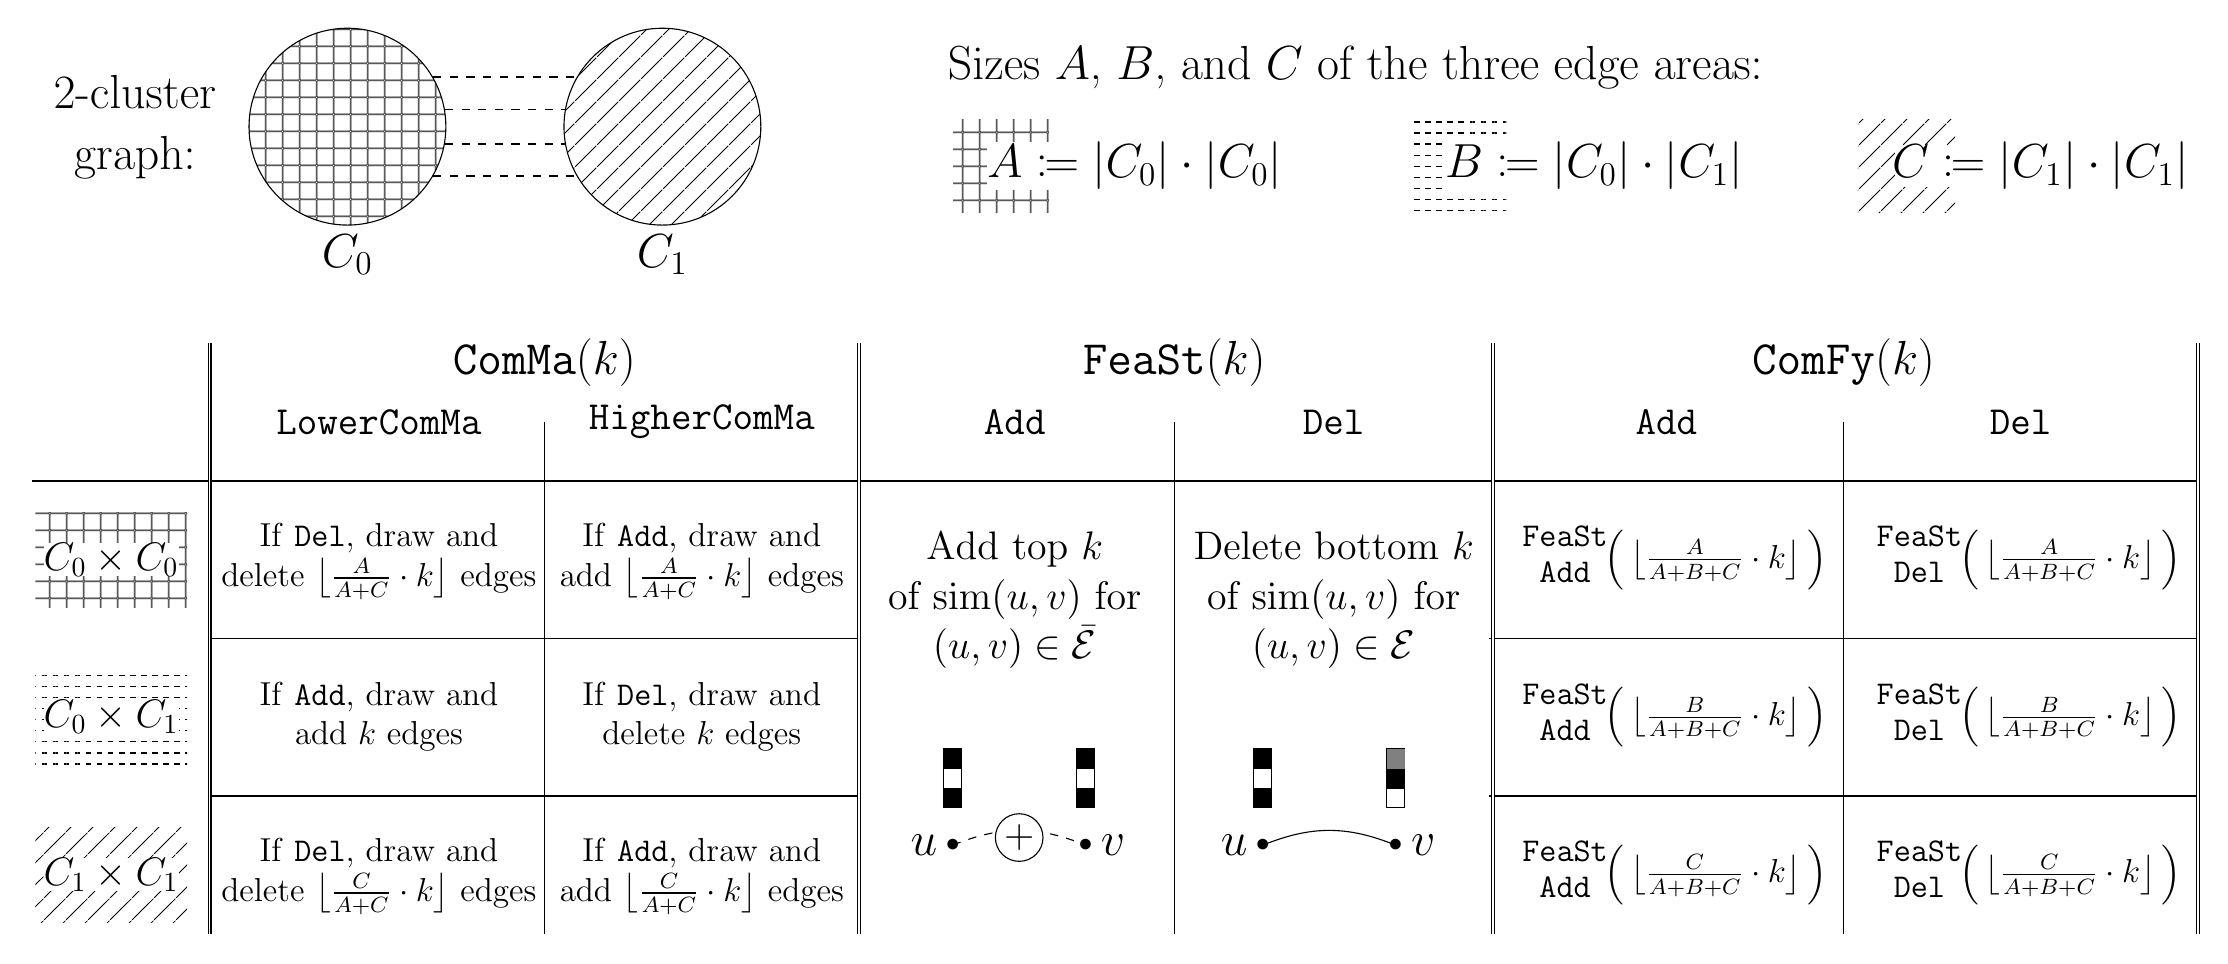
\begin{tikzpicture}

\begin{scope}[xshift=6.5cm,yshift=3.5cm]    
\node[circleA, draw] (A) at (0,0) {};
\node[below=1.25cm] at (A) {\LARGE$C_0$};
\node[circleB, draw] (B) at (4,0) {};
\node[below=1.25cm] at (B) {\LARGE$C_1$};
\draw[connector] (A.30) -- (B.150);
\draw[connector] (A.10) -- (B.170);
\draw[connector] (A.-10) -- (B.190);
\draw[connector] (A.-30) -- (B.210);
\node at (-2.7,0) {\LARGE\begin{tabular}{c}
 2-cluster\\ graph:
\end{tabular}};
\end{scope}
\begin{scope}[xshift=16.5cm,yshift=3cm]
\node[circleA, rectangle,inner sep=12pt,minimum size=0cm] (A1) at (-1.7,0) {\phantom{\Large$A $}};
\node[fill=white,inner sep=0pt] at (0,0) {\LARGE$A \coloneqq |C_0| \cdot|C_0|$};
\node at (2.8,1.25) {\LARGE Sizes $A$, $B$, and $C$ of the three edge areas:};
\end{scope}
\begin{scope}[xshift=22.33cm,yshift=3cm]
\node[circleC, rectangle,inner sep=11pt,minimum size=0cm] (A1) at (-1.7,0.0) {\phantom{\Large$B $}};
\node[fill=white,inner sep=0pt] at (0,0) {\LARGE$B \coloneqq |C_0| \cdot|C_1|$};
\end{scope}
\begin{scope}[xshift=28cm,yshift=3cm]
\node[circleB, rectangle,inner sep=12pt,minimum size=0cm] (A1) at (-1.7,0) {\phantom{\Large$C $}};
\node[fill=white,inner sep=-1pt] at (0,0) {\LARGE$C \coloneqq |C_1| \cdot|C_1|$};
\end{scope}

\begin{scope}[xshift=3.5cm]

\draw (-1,-1) -- (26.5,-1);
\draw (1.25,-3) -- (9.5,-3);\draw (17.5,-3) -- (26.5,-3);
\draw (1.25,-5) -- (9.5,-5);\draw (17.5,-5) -- (26.5,-5);

\node[circleA, inner sep=13pt,minimum size=0cm,rectangle] (A1) at (0,-2) {\phantom{\!\!$C_0\times C_0$\!\!}};
\node[inner sep=0pt,fill=white,rectangle] at (A1) {\Large$C_0\times C_0$};

\node[circleC, inner sep=13pt,minimum size=0cm,rectangle] (B1) at (0,-4)  {\phantom{\!\!$C_0\times C_1$\!\!}};
\node[inner sep=0pt,fill=white,rectangle] at (B1) {\Large$C_0\times C_1$};

\node[circleB, inner sep=13pt,minimum size=0cm,rectangle] (C1) at (0,-6) {\phantom{\!\!$C_1\times C_1$\!\!}};
\node[inner sep=0pt,fill=white,rectangle] at (C1) {\Large$C_1\times C_1$};

\draw[double] (1.25,0.75) -- (1.25,-6.75);
\end{scope}

\begin{scope}[xshift=9cm]
\node at (0,0.5) {\LARGE\texttt{ComMa}($k$)};
\node at (-2.1,-0.25) {\Large\texttt{LowerComMa}};
\node at (-2.1,-2) {\large\begin{tabular}{c}
  If \texttt{Del}, draw and \\
   delete {$\left\lfloor\frac{A}{A+C}\cdot k\right\rfloor$} edges
\end{tabular}
};
\node at (-2.1,-4) {\large\begin{tabular}{c}
  If \texttt{Add}, draw and \\
   add {$k$} edges
\end{tabular}
};
\node at (-2.1,-6) {\large\begin{tabular}{c}
  If \texttt{Del}, draw and \\
   delete {$\left\lfloor\frac{C}{A+C}\cdot k\right\rfloor$} edges
\end{tabular}
};

\draw (0,-0.25) -- (0,-6.75);
\node at (2,-0.25) {\Large\texttt{HigherComMa}};
\node at (2,-2) {\large\begin{tabular}{c}
  If \texttt{Add}, draw and \\
   add {$\left\lfloor\frac{A}{A+C}\cdot k\right\rfloor$} edges
\end{tabular}
};
\node at (2,-4) {\large\begin{tabular}{c}
  If \texttt{Del}, draw and \\
   delete {$k$} edges
\end{tabular}
};
\node at (2,-6) {\large\begin{tabular}{c}
  If \texttt{Add}, draw and \\
   add {$\left\lfloor\frac{C}{A+C}\cdot k\right\rfloor$} edges
\end{tabular}
};

\draw[double] (4,0.75) -- (4,-6.75);
\end{scope}

\begin{scope}[xshift=17cm,xscale=0.9]
\node at (0,0.5) {\LARGE\texttt{FeaSt}($k$)};
\node at (-2.25,-0.25) {\Large\texttt{Add}};
\node at (-2.25,-2.5) {\Large
\begin{tabular}{c}
Add top $k$ \\
of $\text{sim}(u,v)$ for \\
$(u,v) \in \bar{\mathcal{E}}$
\end{tabular}
};

\begin{scope}[scale=1.25,xshift=.5cm,yshift=.5cm]
\node (uNODE) at (-3,-5) {$\bullet$};
\node[left=2pt] at (uNODE) {\LARGE$u$};
\draw[above=25pt] (-3.1,-5.5) -- (-3.1,-4.9) -- (-2.9,-4.9) -- (-2.9,-5.5) -- cycle;
\draw[above=25pt] (-2.9,-5.3) -- (-3.1,-5.3);
\draw[above=25pt] (-2.9,-5.1) -- (-3.1,-5.1);
\fill[above=25pt] (-3.1,-5.5) -- (-3.1,-5.3) -- (-2.9,-5.3) -- (-2.9,-5.5) -- cycle;
\fill[above=25pt] (-3.1,-4.9) -- (-3.1,-5.1) -- (-2.9,-5.1) -- (-2.9,-4.9) -- cycle;

\node (vNODE) at (-1.5,-5) {$\bullet$};
\node[right=2pt] at (vNODE) {\LARGE$v$};
\draw[above=25pt] (-1.6,-5.5) -- (-1.6,-4.9) -- (-1.4,-4.9) -- (-1.4,-5.5) -- cycle;
\draw[above=25pt] (-1.4,-5.3) -- (-1.6,-5.3);
\draw[above=25pt] (-1.4,-5.1) -- (-1.6,-5.1);
\fill[above=25pt] (-1.6,-5.5) -- (-1.6,-5.3) -- (-1.4,-5.3) -- (-1.4,-5.5) -- cycle;
\fill[above=25pt] (-1.6,-4.9) -- (-1.6,-5.1) -- (-1.4,-5.1) -- (-1.4,-4.9) -- cycle;

\draw[dashed] (-3,-5) to[out=20,in=180-20] (-1.5,-5);
\foreach \i in {5} {
\path[below=-3pt] (-3,-5) to[out=30,in=180-30] 
node[pos=0.\i,circle,draw,inner sep=1pt,fill=white]{\Large +} (-1.5,-5);
}
\end{scope}

\draw (0,-0.25) -- (0,-6.75);
\node at (2.25,-0.25) {\Large\texttt{Del}};
\node at (2.25,-2.5) {\Large
\begin{tabular}{c}
 Delete bottom $k$ \\
of $\text{sim}(u,v)$ for \\
$(u,v) \in {\mathcal{E}}$
\end{tabular}};

\begin{scope}[scale=1.25,xshift=-.5cm,yshift=.5cm]
\node (vNODE) at (3,-5) {$\bullet$};
\node[right=2pt] at (vNODE) {\LARGE$v$};
\draw[above=25pt] (3.1,-5.5) -- (3.1,-4.9) -- (2.9,-4.9) -- (2.9,-5.5) -- cycle;
\draw[above=25pt] (2.9,-5.3) -- (3.1,-5.3);
\draw[above=25pt] (2.9,-5.1) -- (3.1,-5.1);
\fill[above=25pt] (3.1,-5.1) -- (3.1,-5.3) -- (2.9,-5.3) -- (2.9,-5.1) -- cycle;
\fill[above=25pt,color=black!50,inner sep=0pt] (3.1,-4.9) -- (3.1,-5.1) -- (2.9,-5.1) -- (2.9,-4.9) -- cycle;

\node (uNODE) at (1.5,-5) {$\bullet$};
\node[left=2pt] at (uNODE) {\LARGE$u$};
\draw[above=25pt] (1.6,-5.5) -- (1.6,-4.9) -- (1.4,-4.9) -- (1.4,-5.5) -- cycle;
\draw[above=25pt] (1.4,-5.3) -- (1.6,-5.3);
\draw[above=25pt] (1.4,-5.1) -- (1.6,-5.1);
\fill[above=25pt] (1.6,-5.5) -- (1.6,-5.3) -- (1.4,-5.3) -- (1.4,-5.5) -- cycle;
\fill[above=25pt] (1.6,-4.9) -- (1.6,-5.1) -- (1.4,-5.1) -- (1.4,-4.9) -- cycle;

\draw (1.5,-5) to[out=20,in=180-20] (3,-5);
\foreach \i in {7} {
\path[above=-3pt] (1.5,-5) to[out=30,in=180-30] 
node[pos=0.\i,rotate=90]{\LARGE\ScissorRight} (3,-5);
}
\end{scope}

\draw[double] (4.5,0.75) -- (4.5,-6.75);
\end{scope}

\begin{scope}[xshift=25.5cm]
\node at (0,0.5) {\LARGE\texttt{ComFy}($k$)};
\node at (-2.25,-0.25) {\Large\texttt{Add}};
\node at (-2.25,-2) {\large\begin{tabular}{c}
 \large\texttt{FeaSt}\\[-1pt]
 \large\texttt{Add}\\[2pt]
\end{tabular}\hspace{-11pt}
$\Big(\left\lfloor\frac{A}{A+B+C}\cdot k\right\rfloor\Big)$};
\node at (-2.25,-4) {\large\begin{tabular}{c}
 \large\texttt{FeaSt}\\[-1pt]
 \large\texttt{Add}\\[2pt]
\end{tabular}\hspace{-11pt}
$\Big(\left\lfloor\frac{B}{A+B+C}\cdot k\right\rfloor\Big)$};
\node at (-2.25,-6) {\large\begin{tabular}{c}
 \large\texttt{FeaSt}\\[-1pt]
 \large\texttt{Add}\\[2pt]
\end{tabular}\hspace{-11pt}
$\Big(\left\lfloor\frac{C}{A+B+C}\cdot k\right\rfloor\Big)$};

\draw (0,-0.25) -- (0,-6.75);
\node at (2.25,-0.25) {\Large\texttt{Del}};
\node at (2.25,-2) {\large\begin{tabular}{c}
 \large\texttt{FeaSt}\\[-1pt]
 \large\texttt{Del}\\[2pt]
\end{tabular}\hspace{-11pt}
$\Big(\left\lfloor\frac{A}{A+B+C}\cdot k\right\rfloor\Big)$};
\node at (2.25,-4) {\large\begin{tabular}{c}
 \large\texttt{FeaSt}\\[-1pt]
 \large\texttt{Del}\\[2pt]
\end{tabular}\hspace{-11pt}
$\Big(\left\lfloor\frac{B}{A+B+C}\cdot k\right\rfloor\Big)$};
\node at (2.25,-6) {\large\begin{tabular}{c}
 \large\texttt{FeaSt}\\[-1pt]
 \large\texttt{Del}\\[2pt]
\end{tabular}\hspace{-11pt}
$\Big(\left\lfloor\frac{C}{A+B+C}\cdot k\right\rfloor\Big)$};

\draw[double] (4.5,0.75) -- (4.5,-6.75);
\end{scope}

\end{tikzpicture}
}
    
    \caption{Behaviour of the proposed algorithms on a 2-cluster graph for $k$ edge modifications. Columns denote our methods and their variants (see \S\ref{s:algs}, \S\ref{app:algs}). Rows indicate 3 edge areas used for budgeting across the graph \textemdash except for \texttt{FeaSt}, which is global. 
    The (latent) clusters are precomputed via Louvain. 
    \texttt{ComMa} randomly draws edges from all intra or all inter-cluster areas, which is equivalent to drawing from each area with a proportional budget in expectation. This insight is translated to \texttt{ComFy}, but the edges are not drawn randomly but prioritized similarly to \texttt{FeaSt}.}
    \label{fig:methods}
\end{figure}
\label{concept}





\subsection{Related work}
\textbf{Graph rewiring.}
A key component for GNNs is the input graph, since it not only acts as the data for model training but is also the computational structure on which \emph{message passing} \citep{quachem} is performed. Real-world graphs, however, can be noisy and sub-optimal for downstream tasks. For example, recent studies have pointed out issues like over-squashing \citep{alon2021on,topping2022understanding,digiovanni2023oversquashing}, caused by topological bottlenecks, which affect how information is diffused. This highlights the importance of the graph topology and begs the question: how can we obtain an optimal computational structure that aligns with the downstream task? Graph rewiring has emerged as a popular technique to effect changes to the edge structure. This can be done based on various criteria. For instance, \citet{topping2022understanding,sjlr,borf} propose to use different variants of Ricci curvature \citep{hamilton} to rewire the graph, while \citet{effectiveresistance} propose the effective resistance \citep{chandraeffective}, and \citet{Banerjee,deac2022expander} transform the input graph into an expander graph \citep{salez2021sparse} for efficient message passing. 
Edges can be added or deleted and even though GNNs should be able to learn to drop task-irrelevant neighbors, trainability and expressiveness issues can limit this ability \citep{mustafa2023are,mustafa2024gate}, which explains why edge deletions can also help fight over-smoothing in addition to over-squashing \citep{jamadandi2024spectral}.

\textbf{Spectral gap maximization.}
Contemporaneously, spectral-based methods such as \citet{Fosr} aim to \textit{maximize} the spectral gap by edge additions, as a larger spectral gap is inherently linked to faster mixing time \citep{mixingtimes} and thus better information flow. However, this can be detrimental in the case of heterophilic graphs \citep{homonecessity,dichotomoy} as we might add edges between nodes of different labels resulting in over-smoothing \citep{li2019deepgcns,NT2019RevisitingGN,ono,zhou2021dirichlet,keriven2022not}. The spectral gap can also be maximized by deleting edges \citep{jamadandi2024spectral} and this has shown to be beneficial in slowing down detrimental over-smoothing while simultaneously mitigating over-squashing, especially in heterophilic settings. Contrarily, \citet{diffwire} advocate for spectral gap \textit{minimization}, but do not explain when this could be advantageous. 

\textbf{Graph and task alignment.}
Our findings reveal that the underlying mechanism enhancing GNN performance by rewiring actually depends on whether we modify edges connecting nodes with similar or dissimilar features, that are usually associated with similar or dissimilar labels. 
In fact, \citet{interplaycommunity} take a first step in this direction by analysing the interplay between community and node-labels. 
They propose an information-theoretic metric, and demonstrate its impact on performance by artificially creating and destroying communities in real-world graphs. This also highlights the importance of the positive influence of same-label neighbours and how different-label neighbours can impair node classification performance \citep{labelawaregcn}.
We take this analysis several steps further and analyze why spectral rewiring cannot induce this alignment (\autoref{th:sbmsgproof}).  

The desirability of alignment between the graph structure and the task in GNNs has been explored in the context of their training dynamics by \citet{yang2024how}. This study theoretically analyzes how GNN models tend to align their Neural Tangent Kernel (NTK) matrix $\mathbf{\Theta}_t$ with the adjacency matrix $A$ of the input graph. 
They further derive a generalization bound for the NTK regime without considering node features, specifically in cases where the adjacency matrix $A$ is well-aligned with the optimal kernel matrix $\mathbf{\Theta}^*$. 
This matrix $\mathbf{\Theta}^*$ precisely indicates whether a pair of nodes share the same label, making this concept of alignment similar to ours \textemdash though not explicitly referring to the graph's communities\textemdash~and to the concept of homophily. 
Our theory on SBMs supports this result on GNN performance, while additionally relating it to the denoising effect of node features by their neighborhoods (\autoref{th:sbmperfproof}) and considering different levels of alignment (\autoref{th:sbmnoiseproof}). 

\subsection{Contributions}
\begin{enumerate}[leftmargin=1.333em]
\item Complementing the graph rewiring literature on spectral gap maximization to fight over-squashing, we highlight real-world cases in which spectral gap minimization is more effective, contrary to conventional approaches. These cases are characterized by high graph-task alignment (when community labels overlap with node labels).
\item Our theoretical insights on SBMs and experimental evidence identify the degree of task and graph structure alignment as the most critical underlying factor to explain when spectral gap rewiring improves a learning task. 
This highlights the major limitation of spectral-based methods, which is that they cannot improve the graph-task alignment directly.
\item To overcome this limitation, motivated by our theoretical insights, we propose to integrate feature similarity into graph rewiring approaches. We explore three novel strategies to study the effect of community structure and feature similarity in isolation (\texttt{ComMa} and \texttt{FeaSt}) and in combination (\texttt{ComFy}). 
\item Extensive real-world experiments confirm our previous insights, highlighting the effectiveness of feature similarity. We find that homophilic graphs tend to benefit most from maximizing global feature similarity \texttt{FeaSt}, while heterophilic graphs {gain} most from a hybrid approach, \texttt{ComFy}, that maximizes feature similarity while respecting the community structure.
\end{enumerate}


\section{Conceptual analysis}


\begin{figure}[t]
  \centering
   \hspace*{0pt}\hfill
    \subfigure[Perfect alignment $\psi=1$.]{%
   \hspace*{0pt}\hfill
\quad\includegraphics[width=4cm]{img/nicematrix1.pdf}
\label{fig:perfalign}\hfill\hspace*{0pt}
}
   \hfill
    \subfigure[Alignment $\psi=\frac{2}{3}$.]{%
  \hspace*{0pt}\hfill
\quad\includegraphics[width=4cm]{img/nicematrix2.pdf}
\label{fig:twothirdsalign}\hfill\hspace*{0pt}
      }
   \hfill\hspace*{0pt}
   
  \caption{Adjacency matrices of $(p,q)$-SBM for different alignments. Shaded areas are intra-community edges drawn with probability $p$ (except self-loops), and unshaded areas are inter-community edges drawn with probability $q$. In Figure~\ref{fig:perfalign}, the two communities match classes $c_1$ (orange) and $c_2$ (purple). In Figure~\ref{fig:twothirdsalign}, a third of nodes in each community are of the opposite class.
  }
  \label{fig:sbmexpl}
\end{figure}

\subsection{Spectral rewiring affects community strength}
Spectral rewiring approaches usually focus on reducing over-squashing by maximizing the spectral gap of the input graph. However, maximizing the gap has a distinct effect on its latent community structure. It is the case that, by maximizing the spectral gap, inter-community edges are added and intra-community edges are deleted, which attenuates the community strength (\autoref{th:sbmsgproof}).

When there is a high graph-task alignment, which has also been termed as the cluster hypothesis \citep{clusterhypothesis}, the addition of inter-community edges likely adds more inter-class edges, while the removal of intra-community edges likely deletes many intra-class edges. 
Consequently, message passing happens on a less informative computational structure, rendering the rewiring detrimental to the performance of any classifier (\autoref{th:sbmperfproof}). 
On the other hand, by minimizing the spectral gap inter-community edges are deleted and intra-community edges are added, which strengthens the community structure. 
If this structure is highly aligned with the labels, the rewiring should be beneficial, as it increases feature similarity of nodes that have the same label, thus making different class nodes better separable.

To make these intuitive statements more rigorous and quantifiable, we relate community structure and node labels in a paradigmatic example of community structure:
the Stochastic Block Model (SBM ($p,q,\mathcal{C}$)), which is a random graph model with planted communities. 
The nodes are partitioned into $\mathcal{C}$ communities \textemdash we adopt a binary SBM ($\mathcal{C} = 2$) unless explicitly stated otherwise. 
We can observe the form of the adjacency matrix of a two-block $(p,q)$ SBM in \autoref{fig:sbmexpl}.
The edges are randomly sampled with probabilities $p$ for intra-community edges and $q$ for inter-community edges. 
Both values critically influence the performance of GNNs on a sampled graph, as they determine the amount of neighborhood aggregation.
High values of $p$ and low values of $q$ lead to a strong, pronounced community structure.
Thus, the node features after message passing tend to become more similar within communities in this setting. 
Similar values of $p \approx q$ would make the community structure difficult to detect and the feature distributions of different communities would not necessarily become more distinguishable after neighborhood aggregation.

To relate this reasoning to spectral gap optimization, we first establish a direct link to the community structure in SBMs.
\begin{theorem}[A less pronounced community structure corresponds to a higher spectral gap]\label{th:sbmsgproof}

	Let $G$ be a ($p$-$q$)-SBM with $N$ nodes in 2 equally-sized communities and intra/inter-edge probabilities $p > q$. 
	Let $G^{\text{del}}$ be a ($p'$-$q$)-SBM where $p'<p$, and $G^{\text{add}}$ be a ($p$-$q'$)-SBM where $q'>q$. The (expected) spectral gap of $G$ is smaller than those of $G^{\text{del}}$ and $G^{\text{add}}$: $\lambda_1(G) < \lambda_1(G^{\text{del}}),$ and $\lambda_1(G) < \lambda_1(G^{\text{add}})$. In fact, the spectral gap grows approximately like $-\frac{p-q}{q+p}$. 
\end{theorem}
In summary, increasing $q$ and decreasing $p$ increases the spectral gap but makes the community structure less pronounced, and vice versa.
The next theorem establishes how this is connected to the performance of a model that performs sum aggregation, which we use as a tractable GNN proxy.
\begin{theorem}[A less pronounced community structure harms performance {\textemdash if high graph-task alignment}] \label{th:sbmperfproof}

Let $G$ be the ($p$-$q$)-SBM from \autoref{th:sbmsgproof}. Let $x_i$ be the single feature of node $i$ {where $x_i\sim\mathcal{N}(-1,1)$ if its class $\ell_i=c_1$ or $x_i\sim\mathcal{N}(1,1)$ if its class $\ell_i=c_2$, and $\ell_i$ corresponds one-to-one} to node $i$'s block membership. Let $f$ be an optimal classifier on the model's features, $X$, and $e(f,X)$ the (expected) proportion of misclassified nodes. After a step of sum aggregation, $e$ is monotonically decreasing with respect to $p$, and increasing with respect to $q$.

\end{theorem}

\subsection{Varying the amount of graph-task alignment} \label{gtalignment}
\autoref{th:sbmperfproof} applies to an SBM with perfect alignment between its clusters and node labels. However, in real-world graphs, this assumption is rarely satisfied. The relationship between the task and the underlying community structure, which might not necessarily be pronounced, can take more complex forms. 
For instance, in heterophilic settings, similar nodes do not need to be connected, so the effect of spectral rewiring on them is not straightforward. 
While spectral rewiring can influence performance by modifying how pronounced the latent community structure is, aggregation on the input graph is much more effective if we improve the mentioned alignment directly, which spectral rewiring fails to do. 

This intuition is corroborated and quantified by our theory. \autoref{th:sbmnoiseproof} describes the behaviour of the proportion of misclassified nodes after a step of neighborhood aggregation.
Let $\psi$ capture the graph-task alignment. An illustration of an SBM with $\psi\neq1$ can be found in Figure~\ref{fig:twothirdsalign}.
If $\psi=1$, we obtain the same behaviour (perfect alignment) as in \autoref{th:sbmperfproof}. 
With $\psi=0$, we obtain an SBM where the node labels are assigned oppositely to their communities, so by renaming the communities we also have perfect alignment. 
For $\psi=0.5$, $P(M) = \Phi(0) = \frac{1}{2}$, so half the nodes are misclassified and this classifier is as good as a random choice.
In this setup, most of the real distributions of neighbours follow binomials. 
For better interpretability, we have simplified the formula with normal approximations to look at the continuous trends. All nuances are derived in the proof (\S\ref{app:sbmnoiseproof}), which suggests that the central $\psi$ parameter controls GNN performance.

\begin{theorem}[The effect of different alignments on performance] \label{th:sbmnoiseproof}
Let $G$ be the ($p$-$q$)-SBM from \autoref{th:sbmsgproof} ($p>q$). Let $x_i$ be the single feature of node $i$ where $x_i\sim\mathcal{N}(-1,1)$ or $x_i\sim\mathcal{N}(1,1)$ depending on its class, and $\ell_i$ its label, which may correspond to node $i$'s block membership with a fixed probability $\psi$. After a step of sum aggregation, the proportion of misclassified nodes of the best classifier $f$ is approximately
$$ P(M)\approx 1-\psi+(2\psi-1) \Phi\left(
\frac{\frac{N}{2} (2 \psi - 1) (p - q)}{\sqrt{\frac{N}{2} ( p+q + p(1-p) + q(1- q)  +  2(p-q)^2\psi(1-\psi) )}}
\right)
$$

\end{theorem}

\subsection{Experiments on SBM for different $p$ and $q$} \label{s:sbmpq}

\begin{figure}[t]
    \centering
     \hfill
    	\subfigure[Correlation of some scores for different values of $(p,q)$.]{\includegraphics[width=0.45\linewidth]{img/corrmatrixsbm.pdf}\label{fig:matrixcorr}}
     \hfill
    	\subfigure[Accuracy of a GCN trained on different $(p,q)$ (averaged for 8 different seeds).]{
     \includegraphics[width=0.45\linewidth]{img/Accuracy-sp.pdf}\label{fig:accssbm}
     }
     \hfill
    \caption{The effects of \autoref{th:sbmsgproof} (for the spectral gap) and Theorems \ref{th:sbmperfproof}, \ref{th:sbmnoiseproof} (for accuracy) on 1000-node SBM-$(p,q)$. Each SBM has different $p$ and $q$, where $p = \{0.5,0.7,0.8,0.99\}$ and $q = \{0.2,0.5\}$, and different alignment between the labels and the communities: $\{0.9,0.95,1\}$, as well as an example of $0.6$ alignment which gets practically null performance. The spectral gap correlates perfectly with $-\frac{p-q}{p+q}$, and negatively with the community structure and the homophily with perfect alignment. Thus, it is equivalent to plot Figure \ref{fig:accssbm} with any of these as the x-axis.}
\end{figure}

The previously stated theorems are also supported by empirical results. 
\autoref{th:sbmsgproof} proves that maximizing the spectral gap results in a weaker latent community structure, while minimization enhances it.
To quantify the impact of the spectral gap on the performance, we sample SBM graphs with normally distributed node features, whose means indicate their class membership.
The class memberships are sampled from independent Bernoulli distributions whose probability (the alignment) depends on a node's community label. 
For different values of $p$ and $q$, we train a 2-layered GCN \citep{Kipf:2017tc} and measure the Normalized Mutual Information (NMI) \citep{supervisedcommunity} between the ground truth labels and the predictions made by the GCN, which we show in Figure \ref{fig:accssbm}.

 Figure \ref{fig:matrixcorr} furthermore validates that the spectral gap correlates with $-\frac{p-q}{q+p}$ and the community strength of the SBM (negatively), as well as with the graph's normalized homophily score \textit{when the alignment is perfect}. When the alignment is weaker, the homophily also decreases homogeneously. In Figure \ref{fig:accssbm}, we compare the spectral gap of these different SBM graphs against the accuracy of a GCN trained on it, using a fixed train-test split.

We find that, in cases of high homophily and high alignment, it is beneficial to minimize the spectral gap, as the communities that get strengthened also correspond to the task labels. 
However, the spectral gap does not completely correlate with the GCN accuracy, as it can only affect the community strength. We can also see that a lack of graph-task alignment reduces the GNN performance, as shown by the different hues in the scatter plot. Changing the alignment only from $1.0$ to $0.95$ reduces dramatically the influence of different $(p,q)$ on the performance. 
But even given a fixed theoretical alignment, the topology of the graph can have nuanced effects on GNN accuracy. 
For instance, the SBM-$(0.5,\ 0.2)$ has a lower spectral gap (and higher homophily) than the SBM-$(0.99,\ 0.5)$, although a worse test performance. 
Yet, the latter has a higher density, which means it is potentially better at denoising and obtaining better separable node representations.
This observation highlights potential benefits resulting from adding edges (and thus increasing the graph density) even without considering feature similarity or graph-task alignments.




\subsection{Analysis of real-world datasets} 

\begin{figure}[t]
    \centering
     \hfill
    \includegraphics[width=0.39\linewidth]{img/coramaxadd.png}
     \hfill
     \includegraphics[width=0.39\linewidth]{img/citeseermaxadd.png}
     \hfill
    \caption{Maximizing the spectral gap (using \citep{jamadandi2024spectral}) on Cora and Citeseer reduces both the graph-task alignment and the test accuracy. {Labels denote the number of edge additions.}}
    \label{fig:coramaxadd}
\end{figure}

Real-world datasets usually have complex community structures and mixed alignment trends. 
Some parts of the graph might show good graph-task alignment while other parts do not invite for spectral-based rewiring.
This makes it difficult to predict when minimization or maximization works best or how many edge modifications are required to see changes in GNN performance. 
On the one hand, very homophilic datasets might be similar to the SBM setup analyzed in the previous theorems, so spectral maximization is detrimental in the long run \textemdash as seen for Cora and Citeseer in \autoref{fig:coramaxadd}, where the alignment between labels and communities gets heavily reduced, and so does the accuracy. 
On the other hand, increasing connectivity might be key for some tasks, where, for example, information needs to travel across different clusters. 
All kinds of spectral rewiring methods can be effective for a small number of edge changes, as they might locally have a denoising effect for some (lucky) edges.


\begin{figure}[t]
    \centering
     \hfill
    	\subfigure[Cora: additions vs. deletions]{\begin{tabular}{cc}
    \includegraphics[width=0.21\linewidth]{img/Cora-MinGap-add-cm.png}
    &
    \includegraphics[width=0.21\linewidth]{img/Cora-MinGap-del-cm.png}
    \\
    \includegraphics[width=0.21\linewidth]{img/Cora-MaxGap-add-cm.png}
    &
    \includegraphics[width=0.21\linewidth]{img/Cora-MaxGap-del-cm.png}
    \\
    \includegraphics[width=0.21\linewidth]{img/Cora-Random-add-cm.png}
    &
    \includegraphics[width=0.21\linewidth]{img/Cora-Random-del-cm.png}
    	\end{tabular}}
     \hfill
    	\subfigure[Chameleon: additions vs. deletions]{\begin{tabular}{cc}
    \includegraphics[width=0.21\linewidth]{img/Chameleon-MinGap-add-cm.png}
    &
    \includegraphics[width=0.21\linewidth]{img/Chameleon-MinGap-del-cm.png}
    \\
    \includegraphics[width=0.21\linewidth]{img/Chameleon-MaxGap-add-cm.png}
    &
    \includegraphics[width=0.21\linewidth]{img/Chameleon-MaxGap-del-cm.png}
    \\
    \includegraphics[width=0.21\linewidth]{img/Chameleon-Random-add-cm.png}
    &
    \includegraphics[width=0.21\linewidth]{img/Chameleon-Random-del-cm.png}
    	\end{tabular}}
     \hfill
    \caption{Alignment matrices for Cora (homophilic) and Chameleon (heterophilic) by a 500-edge rewiring method. In each row: spectral minimization and maximization from \citet{jamadandi2024spectral}, and random rewiring. In each column: additions and deletions. Each alignment matrix compares the number of edges added/deleted in terms of the type of nodes it connects: with the Same or Different L(abel), and with the Same or Different C(ommunity).}
    \label{fig:alignmentmatrix}
\end{figure}

However, the trend variability for spectral rewiring might be explained by the type of edges it adds or deletes, considering both the node and community labels that they connect. 
\autoref{fig:alignmentmatrix} visualizes the number of edges that connect nodes with the same or different node and community labels, for spectral minimization, maximization, and random rewiring of 500 edges, for both Cora and Chameleon. 
We use the spectral gap optimization algorithms presented in  \citet{jamadandi2024spectral}, as they are reliable in maximizing the spectral gap for additions and deletions, and we adapt them for minimization (as described in Algs. \ref{alg:proxyaddmin} and \ref{alg:proxydelmin}). 
The amount of edges for each type clearly changes from the homophilic to the heterophilic case for the different methods. 

In the first row (spectral gap minimization), we see that minimization adds more same-community edges than the other two methods. 
When adding edges in homophilic settings (Cora), this is preferred, because these same-community edges are mostly same-label edges (same C: 152/21). 
However, in heterophilic settings (Chameleon) the opposite is true: making the community structure more pronounced adds edges connecting different labels (same C: 95/265). Deletions are, however, more similar to random rewiring, with the exception of a subtle increase in the pruning of different-community edges for the heterophilic setting, compared to random (Different C: -15/-59).

In the second row (spectral gap maximization), the algorithm exclusively adds different-community edges. 
In homophilic settings, this is detrimental, as most of them will be from different classes (Different C: 36/464). However, in heterophilic settings, often nodes of the same class are connected, which helps align the community structure with the task (different C: 152/348). 
MaxGap also prunes almost exclusively same-community edges, which is again detrimental for the homophilic case (same C: -409/-57) but helps in the heterophilic case (same C: -167/333). 
The fact that spectral maximization by deletions helps especially in heterophilic settings is also supported by its strong benefits for GNN performance \citep{jamadandi2024spectral}.

The alignment matrices serve as a guiding principle to determine if spectral gap maximization or minimization should be preferred. However, spectral gap optimization fails to transform the input graph into a computational structure that is well aligned for the downstream task, which leaves the question, can we do better? 

\section{Graph Rewiring for Community-Node Label Alignment}\label{s:algs}
\textbf{{ComMa}.} 
In our conceptual analysis, we have proven that spectral rewiring algorithms directly affect the community strength of the input graph, and that this can be detrimental to the task when there is an originally good alignment between community and node labels. 
Yet, pre-processing spectral rewiring methods are usually performed in a Greedy manner, and this causes the methods to affect newly obtained community structure but not the original one, which can get lost. 
To obtain clearer insights into the impact of community structure, we propose a non-Greedy and more efficient alternative to spectral rewiring: \texttt{ComMa}. 
This method modifies edges such that they increase or decrease the original community structure directly. The variant that increases community structure is called \texttt{HigherComMa} (Alg. \ref{alg:HigherComMa}), and corresponds to minimizing the spectral gap. 
The method that decreases it is \texttt{LowerComMa} (Alg. \ref{alg:LowerComMa}), and corresponds to maximizing the spectral gap. 
In general, this approach is flexible regarding the method that is applied to detect the community structure of the initial input graph.
We use the Louvain algorithm \citep{Blondel_2008}, as it scales to large graphs and is implemented by the library \textit{nx\_cugraph} for GPU acceleration. The non-accelerated algorithm runs in $O(|\mathcal{V}|\log|\mathcal{V}|)$. 
Rewiring only needs to consider the edges to add ($O(|\bar{\mathcal{E}}|)$) or delete ($O(|{\mathcal{E}}|)$), and to randomly pick a fixed number of them (provided by 
a hyperparameter $N$).

\textbf{{FeaSt}.} 
To make neighborhood aggregation more homogeneous to fight over-smoothing and likely increase homophily, we propose to maximize the pairwise \textit{feature similarity} of all connected nodes in the graph. 
The feature (cosine) similarity between nodes $u$ and $v$ is defined as  $\text{sim}(u,v) = \frac{\langle X_u, X_v\rangle}{\|X_u\|\|X_v\|)}$,
where $X_u, X_v$ are the respective features of nodes $u$ and $v$. 
Although this operation can also be accelerated by GPU, the non-accelerated computation runs in $O(|X_u||\mathcal{V}|^2)$. 
We consider all edges that can be added or deleted, and we rank them according to the similarity, which we would obtain if the edges were added or deleted, respectively. The $N$ modified edges are the top ones of this ranking, which can be obtained in $O(N|\bar{\mathcal{E}}|)$ for additions or $O(N|{\mathcal{E}}|)$ for deletions. The concrete formulas are specified in Alg. \ref{alg:FeaSt}.

\textbf{{ComFy}.} While feature similarity maximization is a well performing pre-processing rewiring approach, it suffers from complementary pitfalls to the spectral rewiring methods. For the latter, it can be disadvantageous to ignore the task. 
For the former (\texttt{FeaSt}), it can be disadvantageous to not account for the original community structure of the graph. Therefore, we propose to restrict the similarity maximization to edges between particular pairs of communities or pairs within a community. 
We call this algorithm \texttt{ComFy} {(Alg. \ref{alg:ComFy})}. In this way, the effect of rewiring is spread across the whole graph, and the original structure is proportionally accounted for. This method still requires to compute all pairwise similarity values, and to detect the graph's original communities. Afterwards, it budgets the number of edges $B_{ij}$ to modify between each pair of communities $(i,j)$ (including intra-community with $i=j$) depending on their \textit{sizes}, and such that the total sum of budgets is approximately $N$. 
For each $(i,j)$, we find the top $B_{ij}$ edges that maximize the similarity of edges bridging them. The complexity of this algorithm is thus comparable to the sum of the other two algorithms.


\section{Experiments}\label{s:experiments}

\begin{table}[t]
\centering
\caption{Accuracy on node classification comparing different rewiring schemes.}
\label{tab:nodeclassificationregular}
\resizebox{\textwidth}{!}{%
\begin{tabular}{cccccccccc}
\toprule
Method          & Cora       & Citeseer   & Pubmed     & Cornell    & Texas      & Wisconsin  & Chameleon           & Squirrel   & Actor      \\ \midrule
GCN        &     86.12±0.36       & 77.83±0.35           &85.57±0.11&    35.14±1.63        &  35.14±1.50          &  38.00±1.47          &    39.33±0.59                 &   31.69±0.42         &   27.24±0.21         \\ 
GCN+BORF        & 87.50±0.20 & 73.80±0.20 & NA         & 50.80±1.10 & NA         & 50.30±0.90 & \textbf{61.50±0.40} & NA         & NA         \\
GCN+FoSR        & 83.50±0.39 & 75.47±0.31 & 86.08±0.10 & 40.54±1.47 & 51.35±1.75 & 54.00±1.46 & 41.01±0.63          & 32.36±0.37 & 27.57±0.21 \\
GCN+ProxyAddMin & 84.10±0.39 & 78.77±0.40 & 86.15±0.10 & 45.95±1.50 & 48.65±1.45 & 42.00±1.23 & 39.33±0.55          & 33.71±0.40 & 28.03±0.22 \\
GCN+ProxyAddMax & 85.92±0.43 & 79.25±0.35 & 86.41±0.11 & 48.65±1.41 & 40.54±1.64 & 50.00±1.25 & 38.20±0.70          & 35.06±0.44 & 25.99±0.20 \\
GCN+ProxyDelMin & 85.92±0.37 & 79.01±0.34 & 86.28±0.11 & 45.95±1.50 & 48.65±1.63 & 44.00±1.13 & 39.89±0.59          & 34.83±0.45 & 26.58±0.25 \\
GCN+ProxyDelMax & 86.32±0.38 & \textbf{81.84±0.38} & 85.95±0.11 & 54.05±1.67 & 48.65±1.35 & 52.00±1.33 & 39.33±0.70          & 34.61±0.39 & 27.30±0.22 \\ \midrule
GCN+HigherComMaAdd & 83.64±0.38 & 77.13±0.38 & 85.86±0.10 & 49.93±1.34 & 52.66±1.47 & 50.55±1.24 & 41.23±0.72          & 34.51±0.40 & 30.92±0.21 \\
GCN+HigherComMaDel & 83.82±0.31 & 77.31±0.41 & 85.90±0.11 & 49.03±1.26 & 48.57±1.53 & 50.32±1.38 & 40.44+0.69          & 34.66±0.39 & 30.71±0.24 \\
GCN+LowerComMaAdd  & 83.41±0.37 & 77.15±0.36 & 85.85±0.09 & 51.08±1.67 & 50.29±1.71 & 50.95±1.29 & 40.61±0.64          & 34.48±0.39 & 30.79±0.23 \\
GCN+LowerComMaDel  & 83.61±0.35 & 77.39±0.37 & 85.90±0.10 & 49.69±1.43 & 50.59±1.52 & 50.61±1.35 & 40.43±0.71          & 34.76±0.40 & 30.79±0.22 \\ \midrule
GCN+FeaStAdd &
  87.73±0.39 &
  78.54±0.34 &
  86.43±0.09 &
  59.46±1.49 &
  54.05±1.51 &
  {60.00±1.09} &
  43.26±0.62 &
  \textbf{39.33±0.73} &
  {31.25±0.22} \\
GCN+FeaStDel &
  \textbf{90.74±0.39} &
  \underline{81.60±0.39} &
  \textbf{86.76±0.10} &
  51.35±1.63 &
  \textbf{64.86±1.43} &
  {60.00±1.27} &
  42.70±0.69 &
  36.40±0.36 &
  \underline{31.97±0.21} \\ \midrule
GCN+ComFyAdd &
  {87.73±0.26} &
  {77.36±0.38} &
  \underline{86.74±0.10} &
  \underline{67.57±1.68} &
  \underline{62.16±1.52} &
  {62.00±1.12} &
  41.57±0.83 &
36.85±0.38 &
\underline{32.30±0.25} \\ 
GCN+ComFyDel &
  {88.13±0.27} &
  {78.07±0.35} &
  {86.23±0.11} &
  \textbf{70.27±1.50}&
  \textbf{64.86±1.51} &
  \textbf{66.00±1.34} &
  \underline{45.51±0.76} &
  \underline{39.10±0.43} &
  31.12±0.19 \\ 
  \bottomrule
\end{tabular}%
}
\end{table}


\begin{table}[t]
\centering
\caption{Node classification on Large Heterophilic Datasets comparing different rewiring schemes.}
\label{tab:nodeclassificationlargehet}
\resizebox{10cm}{!}{%
\begin{tabular}{cccc}
\toprule
Method                   & Roman-Empire        & Amazon-Ratings      & Minesweeper         \\ \midrule
Baseline                 & 70.30±0.73          & 47.20±0.33          & 89.49±0.07          \\
GCN+FoSR                 & 73.60±1.11          & \underline{49.68±0.73}          & 89.66±0.04          \\
GCN+ProxyAddMin          & 79.18±0.06          & 49.30±0.05          & 89.56±0.05          \\
GCN+ProxyAddMax          & 77.54±0.74          & 49.72±0.41          & 89.63±0.05          \\
GCN+ProxyDelMin          & 79.09±0.05          & 49.57±0.06          & 89.60±0.05          \\
GCN+ProxyDelMax          & 77.45±0.68          & \textbf{49.75±0.46} & 89.58±0.04          \\ \midrule
GCN+FeaStAdd       & \textbf{79.67±0.07} & 49.46±0.07          & \underline{89.75±0.05} \\
GCN+FeaStDel       & 78.99±0.05          & 49.19±0.06          & 89.02±0.04          \\
GCN+FeaStAddDel & 79.03±0.07          & 49.39±0.07          & 89.62±0.05          \\  \midrule
GCN+ComFyAdd           &      \underline{79.53±0.07}                &           49.29±0.04          &     \textbf{89.76±0.05}              \\
GCN+ComFyDel         &      79.17±0.07               &            49.21±0.06         &     89.66±0.05                  \\
GCN+ComFyAddDel      &      79.27±0.06               &           49.45±0.07          &                    89.40±0.08 \\ \bottomrule
\end{tabular}%
}
\end{table}


We conduct a comprehensive set of experiments for all proposed algorithms on various benchmark datasets. Our backbone model is GCN \citep{Kipf:2017tc}. Our rewiring techniques could be combined with any GNN model. 
We focus on a simple, common base architecture, as we compare many rewiring techniques in a comparable environment.
Our proposed rewiring algorithms include: \texttt{HigherComMa} which randomly adds/deletes intra-community edges and inter-community edges respectively based on communities detected \citep{modularity,Blondel_2008}; \texttt{LowerComMa} which does the opposite by randomly deleting intra-class edges and adding inter-class edges based on the communities detected; \texttt{FeaSt}, which rewires the graph to maximize the pair-wise cosine similarity between node features; and \texttt{ComFy}, a hybrid version of other two algorithms that uses both the community structure and the feature similarity to rewire the graph. We use the suffixes Add, Delete and AddDel to represent only additions, deletions, or both. Our baselines with which we compare our algorithms are spectral gap maximization methods such as FoSR \citep{Fosr}, ProxyAddMax, and ProxyDelMax proposed in \citet{jamadandi2024spectral}. We further modify the latter algorithms to also \textit{minimize} the spectral gap, resulting in methods ProxyAddMin (Alg. \ref{alg:proxyaddmin}) and ProxyDelMin (Alg. \ref{alg:proxydelmin}). 
The results for the Ricci curvature-based method BORF \citep{borf} is directly taken from their paper \textemdash hence Not Available (NA) for a few datasets. For all tables, the best-performing methods are highlighted in \textbf{bold}, and the second best-performing methods are highlighted with \underline{underlines}. More details on the hyperparameters used are described in \S \ref{app:hyperparams}.

In \autoref{tab:nodeclassificationregular}, we test our algorithms on a variety of homophilic and heterophilic graphs: Cora \citep{Cora}, Citeseer \citep{Citeseer}, Pubmed \citep{Pubmed}, Cornell, Texas, Wisconsin, Chameleon, Squirrel, and Actor \citep{platonov2023critical}. We find that \texttt{FeaSt-Del} performs especially well for homophilic graphs. However,  \texttt{ComFy-Del} seems to be in the lead for the heterophilic ones, and performs comparably for some of the homophilic ones. 
In \autoref{tab:nodeclassificationlargehet} we present the results on accuracy for the large heterophilic graph benchmarks \citep{platonov2023critical} for the spectral rewiring methods, for \texttt{FeaSt} and \texttt{ComFy}. While \texttt{FeaSt-Add} has some good results, all \texttt{ComFy} variants seem to also perform comparably. 
Finally, in \autoref{tab:nodeclassificationregularboth} we present results for both simultaneous additions and deletions for our methods.

\begin{table}[t]
\centering
\caption{Accuracy on node classification with both additions and deletions.}
\label{tab:nodeclassificationregularboth}
\resizebox{\textwidth}{!}{%
\begin{tabular}{cccccccccc}
\toprule
Method       & Cora       & Citeseer   & Pubmed     & Cornell    & Texas      & Wisconsin  & Chameleon           & Squirrel   & Actor      \\ \midrule
GCN     &    86.12±0.36        &   77.83±0.35         &   85.57±0.11         &   35.14±1.63        &      35.14±1.50     &   38.00±1.47         &       39.33±0.59              &  31.69±0.42          &   27.24±0.21         \\
GCN+BORF     & \underline{87.50±0.20} & 73.80±0.20 & NA         & 50.80±1.10 & NA         & 50.30±0.90 & \textbf{61.50±0.40} & NA         & NA         \\ 
GCN+FoSR     & 83.50±0.39 & 75.47±0.31 & 86.08±0.10 & 40.54±1.47 & 51.35±1.75 & 54.00±1.46 & 41.01±0.63          & 32.36±0.37 & 27.57±0.21 \\  \midrule
GCN+HigherComMa & 83.82±0.34 & 77.32±0.38 & 85.83±0.11 & 48.92±1.48 & 52.44±1.64 & 51.35±1.40 & 41.22±0.75          & 34.70±0.40 & 30.81±0.19 \\
GCN+LowerComMa  & 83.76±0.35 & 77.05±0.37 & 85.82±0.10 & 51.46±1.49 & 50.29±1.59 & 50.42±1.27 & 40.49±0.62          & 34.11±0.38 & 30.60±0.22 \\
GCN+FeaSt & 85.71±0.36 & \underline{80.19±0.34} & \underline{87.01±0.12} & \underline{54.05±1.62} & \underline{56.76±1.65} & \underline{58.00±1.26} & 44.94±0.70 & \underline{35.73±0.48} & \underline{32.63±0.21} \\
GCN+ComFy & \textbf{88.93±0.31} & \textbf{80.42±0.46} & \textbf{87.22±0.10} & \textbf{62.16±1.49} & \textbf{59.46±1.68} & \textbf{64.00±1.08} & \underline{46.63±0.69} & \textbf{37.75±0.41}  & \textbf{33.09±0.21} \\
\bottomrule
\end{tabular}%
}
\end{table}

Table \ref{tab:runtimecomparisons} reports the computational efficiency compared to baselines, in seconds, when adding or deleting 50 edges. Concretely, \texttt{ComMa} is orders of magnitude faster than the spectral methods, \texttt{FeaSt} beats most of the baselines, and \texttt{ComFy} is comparable to them. The runtime of methods \texttt{HigherComMa} and \texttt{LowerComMa} are exactly the same, which we denote by \texttt{ComMa}.


\begin{table}[t]
\centering
\caption{Runtime for different rewiring schemes, in seconds, for 50 edges.}
\label{tab:runtimecomparisons}
\resizebox{7cm}{!}{%
\begin{tabular}{@{}ccccc@{}}
\toprule
Method      & Cora & Citeseer & Chameleon & Squirrel \\ \midrule
FoSR        & 4.69 & 5.33     & 5.04      & 19.48    \\
ProxyAddMax & 4.30 & 3.13     & 1.15      & 9.12     \\
ProxyAddMin & 5.03 & 3.63     & 1.08      & 10.01    \\
ProxyDelMax & 1.18 & 0.86     & 1.46      & 7.26     \\
ProxyDelMin & 3.59 & 2.85     & 3.12      & 8.43     \\
ComMaAdd    & 0.05 & 0.03     & 0.04      & 0.63     \\
ComMaDel    & 0.05 & 0.03     & 0.04      & 0.68     \\
FeaStAdd    & 1.78 & 0.92     & 0.56      & 4.43     \\
FeaStDel    & 1.73 & 0.91     & 0.56      & 4.52     \\
ComFyAdd    & 6.29 & 3.85     & 2.84      & 8.72     \\
ComFyDel    & 6.68 & 3.73     & 2.99      & 8.97     \\ \bottomrule
\end{tabular}%
}
\end{table}

\section{Conclusions}
We have introduced three novel graph rewiring techniques —\texttt{ComMa}, \texttt{FeaSt}, and \texttt{ComFy}— designed to improve the performance of Graph Neural Networks (GNNs) by focusing on the alignment between the graph structure and the target task. 

Through our theoretical analysis, we have identified this alignment as a critical factor in explaining performance gains and highlighted it as a major limitation of purely topological-based rewiring strategies that they cannot improve this alignment directly. 
We have discussed this specifically in the context of spectral gap maximization, a widely adopted strategy to address over-squashing, which attenuates the community structure of a graph.
However, when the community labels overlap with the node labels, minimizing the spectral gap (thus amplifying the community structure) would yield significant performance improvements instead.

The basic mechanism behind this improvement is the increase of feature similarity by neighborhood aggregation.
In line with this finding, we have shown that rewiring techniques that explicitly take feature similarity into account, such as \texttt{FeaSt} and \texttt{ComFy}, can lead to significant performance gains, particularly in highly homophilic settings. Our proposed \texttt{ComFy} method, which balances community structure and feature similarity, was shown to outperform spectral rewiring methods in heterophilic settings, where feature alignment across different communities plays a critical role.

Our comprehensive experiments on real-world datasets confirm the effectiveness of these rewiring strategies, demonstrating that a combination of topological and feature-based approaches is key to overcoming the limitations of spectral methods. We believe that this work lays the foundation for future research on task-aware rewiring strategies, and opens the door to more sophisticated methods that leverage both graph topology and node features to optimize GNN performance across a wide range of graph-based applications.


\newpage

\section*{Acknowledgments and Disclosure of Funding}
The authors gratefully acknowledge the Gauss Centre for Supercomputing e.V. for funding this project by providing computing time on the GCS Supercomputer JUWELS at Jülich Supercomputing Centre (JSC). We also gratefully acknowledge funding from the European Research Council (ERC) under the Horizon Europe Framework Programme (HORIZON) for proposal number 101116395 SPARSE-ML.

\bibliographystyle{iclr2025_conference}
\bibliography{iclr2025_conference}
\newpage
\appendix
\section*{Appendix}
\subsection{Lloyd-Max Algorithm}
\label{subsec:Lloyd-Max}
For a given quantization bitwidth $B$ and an operand $\bm{X}$, the Lloyd-Max algorithm finds $2^B$ quantization levels $\{\hat{x}_i\}_{i=1}^{2^B}$ such that quantizing $\bm{X}$ by rounding each scalar in $\bm{X}$ to the nearest quantization level minimizes the quantization MSE. 

The algorithm starts with an initial guess of quantization levels and then iteratively computes quantization thresholds $\{\tau_i\}_{i=1}^{2^B-1}$ and updates quantization levels $\{\hat{x}_i\}_{i=1}^{2^B}$. Specifically, at iteration $n$, thresholds are set to the midpoints of the previous iteration's levels:
\begin{align*}
    \tau_i^{(n)}=\frac{\hat{x}_i^{(n-1)}+\hat{x}_{i+1}^{(n-1)}}2 \text{ for } i=1\ldots 2^B-1
\end{align*}
Subsequently, the quantization levels are re-computed as conditional means of the data regions defined by the new thresholds:
\begin{align*}
    \hat{x}_i^{(n)}=\mathbb{E}\left[ \bm{X} \big| \bm{X}\in [\tau_{i-1}^{(n)},\tau_i^{(n)}] \right] \text{ for } i=1\ldots 2^B
\end{align*}
where to satisfy boundary conditions we have $\tau_0=-\infty$ and $\tau_{2^B}=\infty$. The algorithm iterates the above steps until convergence.

Figure \ref{fig:lm_quant} compares the quantization levels of a $7$-bit floating point (E3M3) quantizer (left) to a $7$-bit Lloyd-Max quantizer (right) when quantizing a layer of weights from the GPT3-126M model at a per-tensor granularity. As shown, the Lloyd-Max quantizer achieves substantially lower quantization MSE. Further, Table \ref{tab:FP7_vs_LM7} shows the superior perplexity achieved by Lloyd-Max quantizers for bitwidths of $7$, $6$ and $5$. The difference between the quantizers is clear at 5 bits, where per-tensor FP quantization incurs a drastic and unacceptable increase in perplexity, while Lloyd-Max quantization incurs a much smaller increase. Nevertheless, we note that even the optimal Lloyd-Max quantizer incurs a notable ($\sim 1.5$) increase in perplexity due to the coarse granularity of quantization. 

\begin{figure}[h]
  \centering
  \includegraphics[width=0.7\linewidth]{sections/figures/LM7_FP7.pdf}
  \caption{\small Quantization levels and the corresponding quantization MSE of Floating Point (left) vs Lloyd-Max (right) Quantizers for a layer of weights in the GPT3-126M model.}
  \label{fig:lm_quant}
\end{figure}

\begin{table}[h]\scriptsize
\begin{center}
\caption{\label{tab:FP7_vs_LM7} \small Comparing perplexity (lower is better) achieved by floating point quantizers and Lloyd-Max quantizers on a GPT3-126M model for the Wikitext-103 dataset.}
\begin{tabular}{c|cc|c}
\hline
 \multirow{2}{*}{\textbf{Bitwidth}} & \multicolumn{2}{|c|}{\textbf{Floating-Point Quantizer}} & \textbf{Lloyd-Max Quantizer} \\
 & Best Format & Wikitext-103 Perplexity & Wikitext-103 Perplexity \\
\hline
7 & E3M3 & 18.32 & 18.27 \\
6 & E3M2 & 19.07 & 18.51 \\
5 & E4M0 & 43.89 & 19.71 \\
\hline
\end{tabular}
\end{center}
\end{table}

\subsection{Proof of Local Optimality of LO-BCQ}
\label{subsec:lobcq_opt_proof}
For a given block $\bm{b}_j$, the quantization MSE during LO-BCQ can be empirically evaluated as $\frac{1}{L_b}\lVert \bm{b}_j- \bm{\hat{b}}_j\rVert^2_2$ where $\bm{\hat{b}}_j$ is computed from equation (\ref{eq:clustered_quantization_definition}) as $C_{f(\bm{b}_j)}(\bm{b}_j)$. Further, for a given block cluster $\mathcal{B}_i$, we compute the quantization MSE as $\frac{1}{|\mathcal{B}_{i}|}\sum_{\bm{b} \in \mathcal{B}_{i}} \frac{1}{L_b}\lVert \bm{b}- C_i^{(n)}(\bm{b})\rVert^2_2$. Therefore, at the end of iteration $n$, we evaluate the overall quantization MSE $J^{(n)}$ for a given operand $\bm{X}$ composed of $N_c$ block clusters as:
\begin{align*}
    \label{eq:mse_iter_n}
    J^{(n)} = \frac{1}{N_c} \sum_{i=1}^{N_c} \frac{1}{|\mathcal{B}_{i}^{(n)}|}\sum_{\bm{v} \in \mathcal{B}_{i}^{(n)}} \frac{1}{L_b}\lVert \bm{b}- B_i^{(n)}(\bm{b})\rVert^2_2
\end{align*}

At the end of iteration $n$, the codebooks are updated from $\mathcal{C}^{(n-1)}$ to $\mathcal{C}^{(n)}$. However, the mapping of a given vector $\bm{b}_j$ to quantizers $\mathcal{C}^{(n)}$ remains as  $f^{(n)}(\bm{b}_j)$. At the next iteration, during the vector clustering step, $f^{(n+1)}(\bm{b}_j)$ finds new mapping of $\bm{b}_j$ to updated codebooks $\mathcal{C}^{(n)}$ such that the quantization MSE over the candidate codebooks is minimized. Therefore, we obtain the following result for $\bm{b}_j$:
\begin{align*}
\frac{1}{L_b}\lVert \bm{b}_j - C_{f^{(n+1)}(\bm{b}_j)}^{(n)}(\bm{b}_j)\rVert^2_2 \le \frac{1}{L_b}\lVert \bm{b}_j - C_{f^{(n)}(\bm{b}_j)}^{(n)}(\bm{b}_j)\rVert^2_2
\end{align*}

That is, quantizing $\bm{b}_j$ at the end of the block clustering step of iteration $n+1$ results in lower quantization MSE compared to quantizing at the end of iteration $n$. Since this is true for all $\bm{b} \in \bm{X}$, we assert the following:
\begin{equation}
\begin{split}
\label{eq:mse_ineq_1}
    \tilde{J}^{(n+1)} &= \frac{1}{N_c} \sum_{i=1}^{N_c} \frac{1}{|\mathcal{B}_{i}^{(n+1)}|}\sum_{\bm{b} \in \mathcal{B}_{i}^{(n+1)}} \frac{1}{L_b}\lVert \bm{b} - C_i^{(n)}(b)\rVert^2_2 \le J^{(n)}
\end{split}
\end{equation}
where $\tilde{J}^{(n+1)}$ is the the quantization MSE after the vector clustering step at iteration $n+1$.

Next, during the codebook update step (\ref{eq:quantizers_update}) at iteration $n+1$, the per-cluster codebooks $\mathcal{C}^{(n)}$ are updated to $\mathcal{C}^{(n+1)}$ by invoking the Lloyd-Max algorithm \citep{Lloyd}. We know that for any given value distribution, the Lloyd-Max algorithm minimizes the quantization MSE. Therefore, for a given vector cluster $\mathcal{B}_i$ we obtain the following result:

\begin{equation}
    \frac{1}{|\mathcal{B}_{i}^{(n+1)}|}\sum_{\bm{b} \in \mathcal{B}_{i}^{(n+1)}} \frac{1}{L_b}\lVert \bm{b}- C_i^{(n+1)}(\bm{b})\rVert^2_2 \le \frac{1}{|\mathcal{B}_{i}^{(n+1)}|}\sum_{\bm{b} \in \mathcal{B}_{i}^{(n+1)}} \frac{1}{L_b}\lVert \bm{b}- C_i^{(n)}(\bm{b})\rVert^2_2
\end{equation}

The above equation states that quantizing the given block cluster $\mathcal{B}_i$ after updating the associated codebook from $C_i^{(n)}$ to $C_i^{(n+1)}$ results in lower quantization MSE. Since this is true for all the block clusters, we derive the following result: 
\begin{equation}
\begin{split}
\label{eq:mse_ineq_2}
     J^{(n+1)} &= \frac{1}{N_c} \sum_{i=1}^{N_c} \frac{1}{|\mathcal{B}_{i}^{(n+1)}|}\sum_{\bm{b} \in \mathcal{B}_{i}^{(n+1)}} \frac{1}{L_b}\lVert \bm{b}- C_i^{(n+1)}(\bm{b})\rVert^2_2  \le \tilde{J}^{(n+1)}   
\end{split}
\end{equation}

Following (\ref{eq:mse_ineq_1}) and (\ref{eq:mse_ineq_2}), we find that the quantization MSE is non-increasing for each iteration, that is, $J^{(1)} \ge J^{(2)} \ge J^{(3)} \ge \ldots \ge J^{(M)}$ where $M$ is the maximum number of iterations. 
%Therefore, we can say that if the algorithm converges, then it must be that it has converged to a local minimum. 
\hfill $\blacksquare$


\begin{figure}
    \begin{center}
    \includegraphics[width=0.5\textwidth]{sections//figures/mse_vs_iter.pdf}
    \end{center}
    \caption{\small NMSE vs iterations during LO-BCQ compared to other block quantization proposals}
    \label{fig:nmse_vs_iter}
\end{figure}

Figure \ref{fig:nmse_vs_iter} shows the empirical convergence of LO-BCQ across several block lengths and number of codebooks. Also, the MSE achieved by LO-BCQ is compared to baselines such as MXFP and VSQ. As shown, LO-BCQ converges to a lower MSE than the baselines. Further, we achieve better convergence for larger number of codebooks ($N_c$) and for a smaller block length ($L_b$), both of which increase the bitwidth of BCQ (see Eq \ref{eq:bitwidth_bcq}).


\subsection{Additional Accuracy Results}
%Table \ref{tab:lobcq_config} lists the various LOBCQ configurations and their corresponding bitwidths.
\begin{table}
\setlength{\tabcolsep}{4.75pt}
\begin{center}
\caption{\label{tab:lobcq_config} Various LO-BCQ configurations and their bitwidths.}
\begin{tabular}{|c||c|c|c|c||c|c||c|} 
\hline
 & \multicolumn{4}{|c||}{$L_b=8$} & \multicolumn{2}{|c||}{$L_b=4$} & $L_b=2$ \\
 \hline
 \backslashbox{$L_A$\kern-1em}{\kern-1em$N_c$} & 2 & 4 & 8 & 16 & 2 & 4 & 2 \\
 \hline
 64 & 4.25 & 4.375 & 4.5 & 4.625 & 4.375 & 4.625 & 4.625\\
 \hline
 32 & 4.375 & 4.5 & 4.625& 4.75 & 4.5 & 4.75 & 4.75 \\
 \hline
 16 & 4.625 & 4.75& 4.875 & 5 & 4.75 & 5 & 5 \\
 \hline
\end{tabular}
\end{center}
\end{table}

%\subsection{Perplexity achieved by various LO-BCQ configurations on Wikitext-103 dataset}

\begin{table} \centering
\begin{tabular}{|c||c|c|c|c||c|c||c|} 
\hline
 $L_b \rightarrow$& \multicolumn{4}{c||}{8} & \multicolumn{2}{c||}{4} & 2\\
 \hline
 \backslashbox{$L_A$\kern-1em}{\kern-1em$N_c$} & 2 & 4 & 8 & 16 & 2 & 4 & 2  \\
 %$N_c \rightarrow$ & 2 & 4 & 8 & 16 & 2 & 4 & 2 \\
 \hline
 \hline
 \multicolumn{8}{c}{GPT3-1.3B (FP32 PPL = 9.98)} \\ 
 \hline
 \hline
 64 & 10.40 & 10.23 & 10.17 & 10.15 &  10.28 & 10.18 & 10.19 \\
 \hline
 32 & 10.25 & 10.20 & 10.15 & 10.12 &  10.23 & 10.17 & 10.17 \\
 \hline
 16 & 10.22 & 10.16 & 10.10 & 10.09 &  10.21 & 10.14 & 10.16 \\
 \hline
  \hline
 \multicolumn{8}{c}{GPT3-8B (FP32 PPL = 7.38)} \\ 
 \hline
 \hline
 64 & 7.61 & 7.52 & 7.48 &  7.47 &  7.55 &  7.49 & 7.50 \\
 \hline
 32 & 7.52 & 7.50 & 7.46 &  7.45 &  7.52 &  7.48 & 7.48  \\
 \hline
 16 & 7.51 & 7.48 & 7.44 &  7.44 &  7.51 &  7.49 & 7.47  \\
 \hline
\end{tabular}
\caption{\label{tab:ppl_gpt3_abalation} Wikitext-103 perplexity across GPT3-1.3B and 8B models.}
\end{table}

\begin{table} \centering
\begin{tabular}{|c||c|c|c|c||} 
\hline
 $L_b \rightarrow$& \multicolumn{4}{c||}{8}\\
 \hline
 \backslashbox{$L_A$\kern-1em}{\kern-1em$N_c$} & 2 & 4 & 8 & 16 \\
 %$N_c \rightarrow$ & 2 & 4 & 8 & 16 & 2 & 4 & 2 \\
 \hline
 \hline
 \multicolumn{5}{|c|}{Llama2-7B (FP32 PPL = 5.06)} \\ 
 \hline
 \hline
 64 & 5.31 & 5.26 & 5.19 & 5.18  \\
 \hline
 32 & 5.23 & 5.25 & 5.18 & 5.15  \\
 \hline
 16 & 5.23 & 5.19 & 5.16 & 5.14  \\
 \hline
 \multicolumn{5}{|c|}{Nemotron4-15B (FP32 PPL = 5.87)} \\ 
 \hline
 \hline
 64  & 6.3 & 6.20 & 6.13 & 6.08  \\
 \hline
 32  & 6.24 & 6.12 & 6.07 & 6.03  \\
 \hline
 16  & 6.12 & 6.14 & 6.04 & 6.02  \\
 \hline
 \multicolumn{5}{|c|}{Nemotron4-340B (FP32 PPL = 3.48)} \\ 
 \hline
 \hline
 64 & 3.67 & 3.62 & 3.60 & 3.59 \\
 \hline
 32 & 3.63 & 3.61 & 3.59 & 3.56 \\
 \hline
 16 & 3.61 & 3.58 & 3.57 & 3.55 \\
 \hline
\end{tabular}
\caption{\label{tab:ppl_llama7B_nemo15B} Wikitext-103 perplexity compared to FP32 baseline in Llama2-7B and Nemotron4-15B, 340B models}
\end{table}

%\subsection{Perplexity achieved by various LO-BCQ configurations on MMLU dataset}


\begin{table} \centering
\begin{tabular}{|c||c|c|c|c||c|c|c|c|} 
\hline
 $L_b \rightarrow$& \multicolumn{4}{c||}{8} & \multicolumn{4}{c||}{8}\\
 \hline
 \backslashbox{$L_A$\kern-1em}{\kern-1em$N_c$} & 2 & 4 & 8 & 16 & 2 & 4 & 8 & 16  \\
 %$N_c \rightarrow$ & 2 & 4 & 8 & 16 & 2 & 4 & 2 \\
 \hline
 \hline
 \multicolumn{5}{|c|}{Llama2-7B (FP32 Accuracy = 45.8\%)} & \multicolumn{4}{|c|}{Llama2-70B (FP32 Accuracy = 69.12\%)} \\ 
 \hline
 \hline
 64 & 43.9 & 43.4 & 43.9 & 44.9 & 68.07 & 68.27 & 68.17 & 68.75 \\
 \hline
 32 & 44.5 & 43.8 & 44.9 & 44.5 & 68.37 & 68.51 & 68.35 & 68.27  \\
 \hline
 16 & 43.9 & 42.7 & 44.9 & 45 & 68.12 & 68.77 & 68.31 & 68.59  \\
 \hline
 \hline
 \multicolumn{5}{|c|}{GPT3-22B (FP32 Accuracy = 38.75\%)} & \multicolumn{4}{|c|}{Nemotron4-15B (FP32 Accuracy = 64.3\%)} \\ 
 \hline
 \hline
 64 & 36.71 & 38.85 & 38.13 & 38.92 & 63.17 & 62.36 & 63.72 & 64.09 \\
 \hline
 32 & 37.95 & 38.69 & 39.45 & 38.34 & 64.05 & 62.30 & 63.8 & 64.33  \\
 \hline
 16 & 38.88 & 38.80 & 38.31 & 38.92 & 63.22 & 63.51 & 63.93 & 64.43  \\
 \hline
\end{tabular}
\caption{\label{tab:mmlu_abalation} Accuracy on MMLU dataset across GPT3-22B, Llama2-7B, 70B and Nemotron4-15B models.}
\end{table}


%\subsection{Perplexity achieved by various LO-BCQ configurations on LM evaluation harness}

\begin{table} \centering
\begin{tabular}{|c||c|c|c|c||c|c|c|c|} 
\hline
 $L_b \rightarrow$& \multicolumn{4}{c||}{8} & \multicolumn{4}{c||}{8}\\
 \hline
 \backslashbox{$L_A$\kern-1em}{\kern-1em$N_c$} & 2 & 4 & 8 & 16 & 2 & 4 & 8 & 16  \\
 %$N_c \rightarrow$ & 2 & 4 & 8 & 16 & 2 & 4 & 2 \\
 \hline
 \hline
 \multicolumn{5}{|c|}{Race (FP32 Accuracy = 37.51\%)} & \multicolumn{4}{|c|}{Boolq (FP32 Accuracy = 64.62\%)} \\ 
 \hline
 \hline
 64 & 36.94 & 37.13 & 36.27 & 37.13 & 63.73 & 62.26 & 63.49 & 63.36 \\
 \hline
 32 & 37.03 & 36.36 & 36.08 & 37.03 & 62.54 & 63.51 & 63.49 & 63.55  \\
 \hline
 16 & 37.03 & 37.03 & 36.46 & 37.03 & 61.1 & 63.79 & 63.58 & 63.33  \\
 \hline
 \hline
 \multicolumn{5}{|c|}{Winogrande (FP32 Accuracy = 58.01\%)} & \multicolumn{4}{|c|}{Piqa (FP32 Accuracy = 74.21\%)} \\ 
 \hline
 \hline
 64 & 58.17 & 57.22 & 57.85 & 58.33 & 73.01 & 73.07 & 73.07 & 72.80 \\
 \hline
 32 & 59.12 & 58.09 & 57.85 & 58.41 & 73.01 & 73.94 & 72.74 & 73.18  \\
 \hline
 16 & 57.93 & 58.88 & 57.93 & 58.56 & 73.94 & 72.80 & 73.01 & 73.94  \\
 \hline
\end{tabular}
\caption{\label{tab:mmlu_abalation} Accuracy on LM evaluation harness tasks on GPT3-1.3B model.}
\end{table}

\begin{table} \centering
\begin{tabular}{|c||c|c|c|c||c|c|c|c|} 
\hline
 $L_b \rightarrow$& \multicolumn{4}{c||}{8} & \multicolumn{4}{c||}{8}\\
 \hline
 \backslashbox{$L_A$\kern-1em}{\kern-1em$N_c$} & 2 & 4 & 8 & 16 & 2 & 4 & 8 & 16  \\
 %$N_c \rightarrow$ & 2 & 4 & 8 & 16 & 2 & 4 & 2 \\
 \hline
 \hline
 \multicolumn{5}{|c|}{Race (FP32 Accuracy = 41.34\%)} & \multicolumn{4}{|c|}{Boolq (FP32 Accuracy = 68.32\%)} \\ 
 \hline
 \hline
 64 & 40.48 & 40.10 & 39.43 & 39.90 & 69.20 & 68.41 & 69.45 & 68.56 \\
 \hline
 32 & 39.52 & 39.52 & 40.77 & 39.62 & 68.32 & 67.43 & 68.17 & 69.30  \\
 \hline
 16 & 39.81 & 39.71 & 39.90 & 40.38 & 68.10 & 66.33 & 69.51 & 69.42  \\
 \hline
 \hline
 \multicolumn{5}{|c|}{Winogrande (FP32 Accuracy = 67.88\%)} & \multicolumn{4}{|c|}{Piqa (FP32 Accuracy = 78.78\%)} \\ 
 \hline
 \hline
 64 & 66.85 & 66.61 & 67.72 & 67.88 & 77.31 & 77.42 & 77.75 & 77.64 \\
 \hline
 32 & 67.25 & 67.72 & 67.72 & 67.00 & 77.31 & 77.04 & 77.80 & 77.37  \\
 \hline
 16 & 68.11 & 68.90 & 67.88 & 67.48 & 77.37 & 78.13 & 78.13 & 77.69  \\
 \hline
\end{tabular}
\caption{\label{tab:mmlu_abalation} Accuracy on LM evaluation harness tasks on GPT3-8B model.}
\end{table}

\begin{table} \centering
\begin{tabular}{|c||c|c|c|c||c|c|c|c|} 
\hline
 $L_b \rightarrow$& \multicolumn{4}{c||}{8} & \multicolumn{4}{c||}{8}\\
 \hline
 \backslashbox{$L_A$\kern-1em}{\kern-1em$N_c$} & 2 & 4 & 8 & 16 & 2 & 4 & 8 & 16  \\
 %$N_c \rightarrow$ & 2 & 4 & 8 & 16 & 2 & 4 & 2 \\
 \hline
 \hline
 \multicolumn{5}{|c|}{Race (FP32 Accuracy = 40.67\%)} & \multicolumn{4}{|c|}{Boolq (FP32 Accuracy = 76.54\%)} \\ 
 \hline
 \hline
 64 & 40.48 & 40.10 & 39.43 & 39.90 & 75.41 & 75.11 & 77.09 & 75.66 \\
 \hline
 32 & 39.52 & 39.52 & 40.77 & 39.62 & 76.02 & 76.02 & 75.96 & 75.35  \\
 \hline
 16 & 39.81 & 39.71 & 39.90 & 40.38 & 75.05 & 73.82 & 75.72 & 76.09  \\
 \hline
 \hline
 \multicolumn{5}{|c|}{Winogrande (FP32 Accuracy = 70.64\%)} & \multicolumn{4}{|c|}{Piqa (FP32 Accuracy = 79.16\%)} \\ 
 \hline
 \hline
 64 & 69.14 & 70.17 & 70.17 & 70.56 & 78.24 & 79.00 & 78.62 & 78.73 \\
 \hline
 32 & 70.96 & 69.69 & 71.27 & 69.30 & 78.56 & 79.49 & 79.16 & 78.89  \\
 \hline
 16 & 71.03 & 69.53 & 69.69 & 70.40 & 78.13 & 79.16 & 79.00 & 79.00  \\
 \hline
\end{tabular}
\caption{\label{tab:mmlu_abalation} Accuracy on LM evaluation harness tasks on GPT3-22B model.}
\end{table}

\begin{table} \centering
\begin{tabular}{|c||c|c|c|c||c|c|c|c|} 
\hline
 $L_b \rightarrow$& \multicolumn{4}{c||}{8} & \multicolumn{4}{c||}{8}\\
 \hline
 \backslashbox{$L_A$\kern-1em}{\kern-1em$N_c$} & 2 & 4 & 8 & 16 & 2 & 4 & 8 & 16  \\
 %$N_c \rightarrow$ & 2 & 4 & 8 & 16 & 2 & 4 & 2 \\
 \hline
 \hline
 \multicolumn{5}{|c|}{Race (FP32 Accuracy = 44.4\%)} & \multicolumn{4}{|c|}{Boolq (FP32 Accuracy = 79.29\%)} \\ 
 \hline
 \hline
 64 & 42.49 & 42.51 & 42.58 & 43.45 & 77.58 & 77.37 & 77.43 & 78.1 \\
 \hline
 32 & 43.35 & 42.49 & 43.64 & 43.73 & 77.86 & 75.32 & 77.28 & 77.86  \\
 \hline
 16 & 44.21 & 44.21 & 43.64 & 42.97 & 78.65 & 77 & 76.94 & 77.98  \\
 \hline
 \hline
 \multicolumn{5}{|c|}{Winogrande (FP32 Accuracy = 69.38\%)} & \multicolumn{4}{|c|}{Piqa (FP32 Accuracy = 78.07\%)} \\ 
 \hline
 \hline
 64 & 68.9 & 68.43 & 69.77 & 68.19 & 77.09 & 76.82 & 77.09 & 77.86 \\
 \hline
 32 & 69.38 & 68.51 & 68.82 & 68.90 & 78.07 & 76.71 & 78.07 & 77.86  \\
 \hline
 16 & 69.53 & 67.09 & 69.38 & 68.90 & 77.37 & 77.8 & 77.91 & 77.69  \\
 \hline
\end{tabular}
\caption{\label{tab:mmlu_abalation} Accuracy on LM evaluation harness tasks on Llama2-7B model.}
\end{table}

\begin{table} \centering
\begin{tabular}{|c||c|c|c|c||c|c|c|c|} 
\hline
 $L_b \rightarrow$& \multicolumn{4}{c||}{8} & \multicolumn{4}{c||}{8}\\
 \hline
 \backslashbox{$L_A$\kern-1em}{\kern-1em$N_c$} & 2 & 4 & 8 & 16 & 2 & 4 & 8 & 16  \\
 %$N_c \rightarrow$ & 2 & 4 & 8 & 16 & 2 & 4 & 2 \\
 \hline
 \hline
 \multicolumn{5}{|c|}{Race (FP32 Accuracy = 48.8\%)} & \multicolumn{4}{|c|}{Boolq (FP32 Accuracy = 85.23\%)} \\ 
 \hline
 \hline
 64 & 49.00 & 49.00 & 49.28 & 48.71 & 82.82 & 84.28 & 84.03 & 84.25 \\
 \hline
 32 & 49.57 & 48.52 & 48.33 & 49.28 & 83.85 & 84.46 & 84.31 & 84.93  \\
 \hline
 16 & 49.85 & 49.09 & 49.28 & 48.99 & 85.11 & 84.46 & 84.61 & 83.94  \\
 \hline
 \hline
 \multicolumn{5}{|c|}{Winogrande (FP32 Accuracy = 79.95\%)} & \multicolumn{4}{|c|}{Piqa (FP32 Accuracy = 81.56\%)} \\ 
 \hline
 \hline
 64 & 78.77 & 78.45 & 78.37 & 79.16 & 81.45 & 80.69 & 81.45 & 81.5 \\
 \hline
 32 & 78.45 & 79.01 & 78.69 & 80.66 & 81.56 & 80.58 & 81.18 & 81.34  \\
 \hline
 16 & 79.95 & 79.56 & 79.79 & 79.72 & 81.28 & 81.66 & 81.28 & 80.96  \\
 \hline
\end{tabular}
\caption{\label{tab:mmlu_abalation} Accuracy on LM evaluation harness tasks on Llama2-70B model.}
\end{table}

%\section{MSE Studies}
%\textcolor{red}{TODO}


\subsection{Number Formats and Quantization Method}
\label{subsec:numFormats_quantMethod}
\subsubsection{Integer Format}
An $n$-bit signed integer (INT) is typically represented with a 2s-complement format \citep{yao2022zeroquant,xiao2023smoothquant,dai2021vsq}, where the most significant bit denotes the sign.

\subsubsection{Floating Point Format}
An $n$-bit signed floating point (FP) number $x$ comprises of a 1-bit sign ($x_{\mathrm{sign}}$), $B_m$-bit mantissa ($x_{\mathrm{mant}}$) and $B_e$-bit exponent ($x_{\mathrm{exp}}$) such that $B_m+B_e=n-1$. The associated constant exponent bias ($E_{\mathrm{bias}}$) is computed as $(2^{{B_e}-1}-1)$. We denote this format as $E_{B_e}M_{B_m}$.  

\subsubsection{Quantization Scheme}
\label{subsec:quant_method}
A quantization scheme dictates how a given unquantized tensor is converted to its quantized representation. We consider FP formats for the purpose of illustration. Given an unquantized tensor $\bm{X}$ and an FP format $E_{B_e}M_{B_m}$, we first, we compute the quantization scale factor $s_X$ that maps the maximum absolute value of $\bm{X}$ to the maximum quantization level of the $E_{B_e}M_{B_m}$ format as follows:
\begin{align}
\label{eq:sf}
    s_X = \frac{\mathrm{max}(|\bm{X}|)}{\mathrm{max}(E_{B_e}M_{B_m})}
\end{align}
In the above equation, $|\cdot|$ denotes the absolute value function.

Next, we scale $\bm{X}$ by $s_X$ and quantize it to $\hat{\bm{X}}$ by rounding it to the nearest quantization level of $E_{B_e}M_{B_m}$ as:

\begin{align}
\label{eq:tensor_quant}
    \hat{\bm{X}} = \text{round-to-nearest}\left(\frac{\bm{X}}{s_X}, E_{B_e}M_{B_m}\right)
\end{align}

We perform dynamic max-scaled quantization \citep{wu2020integer}, where the scale factor $s$ for activations is dynamically computed during runtime.

\subsection{Vector Scaled Quantization}
\begin{wrapfigure}{r}{0.35\linewidth}
  \centering
  \includegraphics[width=\linewidth]{sections/figures/vsquant.jpg}
  \caption{\small Vectorwise decomposition for per-vector scaled quantization (VSQ \citep{dai2021vsq}).}
  \label{fig:vsquant}
\end{wrapfigure}
During VSQ \citep{dai2021vsq}, the operand tensors are decomposed into 1D vectors in a hardware friendly manner as shown in Figure \ref{fig:vsquant}. Since the decomposed tensors are used as operands in matrix multiplications during inference, it is beneficial to perform this decomposition along the reduction dimension of the multiplication. The vectorwise quantization is performed similar to tensorwise quantization described in Equations \ref{eq:sf} and \ref{eq:tensor_quant}, where a scale factor $s_v$ is required for each vector $\bm{v}$ that maps the maximum absolute value of that vector to the maximum quantization level. While smaller vector lengths can lead to larger accuracy gains, the associated memory and computational overheads due to the per-vector scale factors increases. To alleviate these overheads, VSQ \citep{dai2021vsq} proposed a second level quantization of the per-vector scale factors to unsigned integers, while MX \citep{rouhani2023shared} quantizes them to integer powers of 2 (denoted as $2^{INT}$).

\subsubsection{MX Format}
The MX format proposed in \citep{rouhani2023microscaling} introduces the concept of sub-block shifting. For every two scalar elements of $b$-bits each, there is a shared exponent bit. The value of this exponent bit is determined through an empirical analysis that targets minimizing quantization MSE. We note that the FP format $E_{1}M_{b}$ is strictly better than MX from an accuracy perspective since it allocates a dedicated exponent bit to each scalar as opposed to sharing it across two scalars. Therefore, we conservatively bound the accuracy of a $b+2$-bit signed MX format with that of a $E_{1}M_{b}$ format in our comparisons. For instance, we use E1M2 format as a proxy for MX4.

\begin{figure}
    \centering
    \includegraphics[width=1\linewidth]{sections//figures/BlockFormats.pdf}
    \caption{\small Comparing LO-BCQ to MX format.}
    \label{fig:block_formats}
\end{figure}

Figure \ref{fig:block_formats} compares our $4$-bit LO-BCQ block format to MX \citep{rouhani2023microscaling}. As shown, both LO-BCQ and MX decompose a given operand tensor into block arrays and each block array into blocks. Similar to MX, we find that per-block quantization ($L_b < L_A$) leads to better accuracy due to increased flexibility. While MX achieves this through per-block $1$-bit micro-scales, we associate a dedicated codebook to each block through a per-block codebook selector. Further, MX quantizes the per-block array scale-factor to E8M0 format without per-tensor scaling. In contrast during LO-BCQ, we find that per-tensor scaling combined with quantization of per-block array scale-factor to E4M3 format results in superior inference accuracy across models. 


\end{document}
